%%%%%%%%%%%%%%%%%%%%%%%%%%%%%%%%%%%%%%%%%
% Masters/Doctoral Thesis 
% LaTeX Template
% Version 2.5 (27/8/17)
%
% This template was downloaded from:
% http://www.LaTeXTemplates.com
%
% Version 2.x major modifications by:
% Vel (vel@latextemplates.com)
%
% This template is based on a template by:
% Steve Gunn (http://users.ecs.soton.ac.uk/srg/softwaretools/document/templates/)
% Sunil Patel (http://www.sunilpatel.co.uk/thesis-template/)
%
% Template license:
% CC BY-NC-SA 3.0 (http://creativecommons.org/licenses/by-nc-sa/3.0/)
%
%%%%%%%%%%%%%%%%%%%%%%%%%%%%%%%%%%%%%%%%%

%----------------------------------------------------------------------------------------
%	PACKAGES AND OTHER DOCUMENT CONFIGURATIONS
%----------------------------------------------------------------------------------------
\RequirePackage[reqno]{amsmath}
\documentclass[
11pt, % The default document font size, options: 10pt, 11pt, 12pt
%oneside, % Two side (alternating margins) for binding by default, uncomment to switch to one side
english, % ngerman for German
singlespacing, % Single line spacing, alternatives: onehalfspacing or doublespacing
%draft, % Uncomment to enable draft mode (no pictures, no links, overfull hboxes indicated)
%nolistspacing, % If the document is onehalfspacing or doublespacing, uncomment this to set spacing in lists to single
%liststotoc, % Uncomment to add the list of figures/tables/etc to the table of contents
%toctotoc, % Uncomment to add the main table of contents to the table of contents
%parskip, % Uncomment to add space between paragraphs
%nohyperref, % Uncomment to not load the hyperref package
headsepline, % Uncomment to get a line under the header
%chapterinoneline, % Uncomment to place the chapter title next to the number on one line
%consistentlayout, % Uncomment to change the layout of the declaration, abstract and acknowledgements pages to match the default layout
]{MastersDoctoralThesis} % The class file specifying the document structure
\usepackage{minted}
\usepackage{subcaption}
\usepackage{pdflscape}
% \usepackage{listings}
% \usepackage{pythonhighlight}

\usepackage[utf8]{inputenc} % Required for inputting international characters
\usepackage[T1]{fontenc} % Output font encoding for international characters
\usepackage{mathtools}
\usepackage{mathpazo} % Use the Palatino font by default
\usepackage[backend=bibtex,style=numeric,natbib=true]{biblatex} % Use the bibtex backend with the authoryear citation style (which resembles APA)

%\usepackage[backend=bibtex,style=authoryear,natbib=true]{biblatex} % Use the bibtex backend with the authoryear citation style (which resembles APA)

\addbibresource{bibliography.bib} % The filename of the bibliography

\usepackage[autostyle=true]{csquotes} 

\def\HPCsys{\textit{HPC.FASSR}\,}  %%optional: Hydra

%----------------------------------------------------------------------------------------
%	MARGIN SETTINGS
%----------------------------------------------------------------------------------------

\geometry{
	paper=a4paper, % Change to letterpaper for US letter
	inner=2.5cm, % Inner margin
	outer=3.8cm, % Outer margin
	bindingoffset=.5cm, % Binding offset
	top=1.5cm, % Top margin
	bottom=1.5cm, % Bottom margin
	%showframe, % Uncomment to show how the type block is set on the page
}

%----------------------------------------------------------------------------------------
%	THESIS INFORMATION
%----------------------------------------------------------------------------------------

\thesistitle{Improving object management in HPC workflows} % Your thesis title, this is used in the title and abstract, print it elsewhere with \ttitle
\supervisor{Dra. Rosa Maria \textsc{Badia Sala}} % Your supervisor's name, this is used in the title page, print it elsewhere with \supname
\examiner{} % Your examiner's name, this is not currently used anywhere in the template, print it elsewhere with \examname
\degree{Master in Innovation and Research in Informatics} % Your degree name, this is used in the title page and abstract, print it elsewhere with \degreename
\author{Sergio \textsc{Rodríguez Guasch}} % Your name, this is used in the title page and abstract, print it elsewhere with \authorname
\addresses{} % Your address, this is not currently used anywhere in the template, print it elsewhere with \addressname

\subject{Computer Sciences} % Your subject area, this is not currently used anywhere in the template, print it elsewhere with \subjectname
\keywords{} % Keywords for your thesis, this is not currently used anywhere in the template, print it elsewhere with \keywordnames
\university{\href{https://www.upc.edu}{Polytechnic University of Catalonia (UPC) - BarcelonaTech}} % Your university's name and URL, this is used in the title page and abstract, print it elsewhere with \univname
\department{} % Your department's name and URL, this is used in the title page and abstract, print it elsewhere with \deptname
\group{} % Your research group's name and URL, this is used in the title page, print it elsewhere with \groupname
\faculty{\href{https://www.fib.upc.edu/}{Barcelona School of Informatics (FIB)}} % Your faculty's name and URL, this is used in the title page and abstract, print it elsewhere with \facname

\AtBeginDocument{
\hypersetup{pdftitle=\ttitle} % Set the PDF's title to your title
\hypersetup{pdfauthor=\authorname} % Set the PDF's author to your name
\hypersetup{pdfkeywords=\keywordnames} % Set the PDF's keywords to your keywords
}

\begin{document}

\frontmatter % Use roman page numbering style (i, ii, iii, iv...) for the pre-content pages

\pagestyle{plain} % Default to the plain heading style until the thesis style is called for the body content

%----------------------------------------------------------------------------------------
%	TITLE PAGE
%----------------------------------------------------------------------------------------

\begin{titlepage}
\begin{minipage}[c]{0.4\linewidth}
\hspace{0.12\linewidth}%

\includegraphics[keepaspectratio, width=0.76\linewidth]{figures/UPC.png}
\end{minipage}%
\hspace{0.1\linewidth}%
\begin{minipage}[c]{0.4\linewidth}

\includegraphics[keepaspectratio, width=\linewidth]{figures/FIB.png}
\end{minipage}
\begin{center}

\vspace*{.06\textheight}
{\scshape\LARGE \univname\par}\vspace{1.5cm} % University name
\textsc{\Large Master Thesis}\\[0.5cm] % Thesis type

\HRule \\[0.4cm] % Horizontal line
{\huge \bfseries \ttitle\par}\vspace{0.4cm} % Thesis title
\HRule \\[1.5cm] % Horizontal line
 
\begin{minipage}[t]{0.4\textwidth}
\begin{flushleft} \large
\emph{Author:}\\{\authorname} % Author name - remove the \href bracket to remove the link
\end{flushleft}
\end{minipage}
\begin{minipage}[t]{0.4\textwidth}
\begin{flushright} \large
\emph{Supervisor:} \\
{\supname} % Supervisor name - remove the \href bracket to remove the link  
\end{flushright}
\end{minipage}\\[3cm]
 
\vfill

\large \textit{A thesis submitted in fulfillment of the requirements\\ for the degree of \degreename}\\[0.3cm] % University requirement text
\textit{in the}\\[0.4cm]
\facname\\[2cm] % Research group name and department name
 
\vfill
% Defense Date: \\
{\large \today}\\[4cm] % Date


\vfill
\end{center}
\end{titlepage}

%----------------------------------------------------------------------------------------
%	DECLARATION PAGE
%----------------------------------------------------------------------------------------

\begin{declaration}
\addchaptertocentry{\authorshipname} % Add the declaration to the table of contents
\noindent I, \authorname, declare that this thesis titled, \enquote{\ttitle} and the work presented in it are my own. I confirm that:

\begin{itemize} 
\item This work was done wholly or mainly while in candidature for a master degree at this University.
\item Where any part of this thesis has previously been submitted for a degree or any other qualification at this University or any other institution, this has been clearly stated.
\item Where I have consulted the published work of others, this is always clearly attributed.
\item Where I have quoted from the work of others, the source is always given. With the exception of such quotations, this thesis is entirely my own work.
\item I have acknowledged all main sources of help.
\item Where the thesis is based on work done by myself jointly with others, I have made clear exactly what was done by others and what I have contributed myself.
\end{itemize}
 
\noindent Signed:\\
\rule[0.5em]{25em}{0.5pt} % This prints a line for the signature
 
\noindent Date:\\
\rule[0.5em]{25em}{0.5pt} % This prints a line to write the date
\end{declaration}

\cleardoublepage

%----------------------------------------------------------------------------------------
%	QUOTATION PAGE
%----------------------------------------------------------------------------------------

\vspace*{0.2\textheight}

\noindent\enquote{\itshape Love is better than hate, because it brings harmony instead of conflict into the desires of the persons concerned. Two people between whom there is love succeed or fail together, but when two people hate each other the success of either is the failure of the other.}\bigbreak

\hfill Bertrand Russell

%----------------------------------------------------------------------------------------
%	ABSTRACT PAGE
%----------------------------------------------------------------------------------------

\begin{abstract}
\addchaptertocentry{\abstractname} % Add the abstract to the table of contents
Object management represents a substantial fraction of the total computing time in any distributed application, and it also adds complexity in terms of source code. This project proposes and implements a set of features aimed to improve both the usability and performance of distributed applications with heavy object management in task-based parallel and distributed programming models.
\end{abstract}

%----------------------------------------------------------------------------------------
%	ACKNOWLEDGEMENTS
%----------------------------------------------------------------------------------------

\begin{acknowledgements}
\addchaptertocentry{\acknowledgementname} % Add the acknowledgements to the table of contents
I would like to thank the whole Workflows and Distributed Systems team for their patience and help, especially Francesc Lordan for guiding me through the complex maze of the COMPSs Runtime. I am also very grateful to Pol Álvarez, Cristián Ramón-Cortés and Ramón Amela for their help, kindness, knowledge and their almost inhuman ability for dealing with my rants, which were not uncommon.\\
\\
Besides my research team, I would like to express my sincere gratitude and love to Clara, my girlfriend. If it is hard to deal with me at work, just imagine what it is like to live with me.\\
\\
Finally, I also want to thank my family. Thanks for everything. Jero, we will never forget you.
\end{acknowledgements}

%----------------------------------------------------------------------------------------
%	LIST OF CONTENTS/FIGURES/TABLES PAGES
%----------------------------------------------------------------------------------------

\tableofcontents % Prints the main table of contents

\listoffigures % Prints the list of figures

\listoftables % Prints the list of tables

%----------------------------------------------------------------------------------------
%	ABBREVIATIONS
%----------------------------------------------------------------------------------------

%----------------------------------------------------------------------------------------
%	PHYSICAL CONSTANTS/OTHER DEFINITIONS
%----------------------------------------------------------------------------------------

% \begin{constants}{lr@{${}={}$}l} % The list of physical constants is a three column table

% % The \SI{}{} command is provided by the siunitx package, see its documentation for instructions on how to use it

% Speed of Light & $c_{0}$ & \SI{2.99792458e8}{\meter\per\second} (exact)\\
% %Constant Name & $Symbol$ & $Constant Value$ with units\\

% \end{constants}

%----------------------------------------------------------------------------------------
%	SYMBOLS
%----------------------------------------------------------------------------------------

% \begin{symbols}{lll} % Include a list of Symbols (a three column table)

% % $a$ & distance & \si{\meter} \\
% % $P$ & power & \si{\watt} (\si{\joule\per\second}) \\
% %Symbol & Name & Unit \\

% \addlinespace % Gap to separate the Roman symbols from the Greek

% $\mu$ & population mean &  \\
% $\sigma$ &  standard deviation &  \\

% \end{symbols}

%----------------------------------------------------------------------------------------
%	DEDICATION
%----------------------------------------------------------------------------------------


%----------------------------------------------------------------------------------------
%	THESIS CONTENT - CHAPTERS
%----------------------------------------------------------------------------------------

\mainmatter % Begin numeric (1,2,3...) page numbering

\pagestyle{thesis} % Return the page headers back to the "thesis" style

\chapter{Introduction}
\label{sec:introduction}

\section{Motivation}
\label{subsec:intro_motivation}
Most modern research fields use computational resources in some way or another. This trend started some decades ago, and it seems to be increasingly accepted and adopted among all the scientific fields. While computer science contributed to solve many research problems, it also created new challenges to researchers, as the increasing difficulty on programming and software development due to the increasing sizes of data sets, experiments, and number and complexity of the available computational resources. This problem becomes even more noticeable when a research group has no computer scientists and all the programming tasks are done by non-experts. This happens to be very common in fields like biology, chemistry or physics.\\
\\
\textit{Non-expert} programming has always been an issue, but it was far more manageable when all the programs ran sequentially in a single core machine. Multi-core CPUs allowed a program to run various fragments of its code at the same time and thus increased the difficulty of programming both in a conceptual and in a technical way. Parallel programming introduced concepts such as \textit{race condition}, \textit{data dependency}, \textit{critical region}, \textit{parallelism factor}, \textit{granularity}, \textit{overhead} and many more, and the existing frameworks (e.g: native threads) were too low level to be understood or used by non computer scientists, and implied high development and maintainment costs.\\
\\
This shift towards more complex computational models and programs due to the presence of parallelism encouraged the industry to create easier frameworks and programming models for parallel computing. One of the greatest examples of these new frameworks is OpenMP\cite{openmp08}. OpenMP simplified the task of writing parallel programs a lot, making it understandable to non computer scientists. As an example, a working sequential matrix multiplication algorithm can be written as follows:
\inputminted{c}{snippets/matmul_openmp.cc}
Note that all the forks, joins, private copies and similar are just \textit{specified}, but not done explicitly. This simplification allowed the general programming public to take advantage of parallelism. There are many other concurrent and parallel frameworks and models, such as MPI\cite{Forum:1994:MMI:898758}, and many programming languages, such as Java, have a built-in threading library, which is usually simpler to use than native, low-level threads. Even some languages, such as Erlang, are explicitly designed for concurrent and parallel programming.\\
\\
For many years the computational \textit{growth model} consisted of simply adding more resources to increase the potential degree of parallelism, as the performance improvements of individual processors stagnated. In last years, the parallel growth model also started to show signs of stagnation, but the demand of computational resources and the size of the problems to solve are still increasing. In fact, the sizes of the datasets experimented an exponential growth with the boom of paradigms such as Big Data or Deep Learning, in which it is not strange to deal with datasets that, simply put, do not fit in a single machine.\\
\\
So, the next step was obvious: make a program run in different machines simultaneously. This implied many new challenges, such as having many different memories and therefore many different versions of the same object allocated in machines with possibly different architectures. Some other problems appeared, as the impossibility to know the exact order in which events happened in a single program, as different machines have different clocks \cite{Lamport}, making the task of debugging this kind of programs even harder. The previous problems from parallel programming were inherited or got even worse. Data dependencies, race conditions, and the importance of granularity are still there. Some algorithms are much harder to implement in a distributed fashion due to not having the whole input available at the same time, but only pieces or chunks of it. Also, software developers are now forced to take into account an extra level of parallelism when designing their applications if they want to take advantage of all the available resources.\\
\\
As happened with parallel programming, the demands of the industry encouraged the development of frameworks, programming models and file systems aimed to make the development of distributed applications easier. These frameworks and programming models usually abstract the user from things such as explicit computational resource management, synchronization between processes, logging, and network and object handling.\\
\\
One of the most used frameworks is Spark \cite{Zaharia:2010:SCC:1863103.1863113} alongside with HDF5 \cite{shvachko2010hadoop}. Usually, a Spark application consists of the repeated application of a set of fixed patterns, such as map-reduce, while making the \textit{hard steps} transparent to the user. Although this is a very powerful tool, it still requires a strong programming knowledge, as it may not be trivial to translate any idea or an already existing application to this set of patterns. It is for this reason that task-based programming models offer a good alternative. A task-based programming model lets the user to select which parts of the code will be tasks, allowing him to take already existing applications and make them run in a distributed environment with minimal effort.

\section{Objectives}
\label{subsec:intro_objectives}
This project focuses on improving the task-based programming model COMP Superscalar (and, from now on, COMPSs) \cite{compss} by both adding features aimed to improve usability and performance by focusing on the object management stage. Object management implies a lot of different algorithms and computational problems. Some of them are:
\begin{itemize}
\item Have a quick way to uniquely identify user objects
\item Translate user objects into something transferable between different machines with, possibly, different architectures and/or versions of some of its software. Try to cover as much objects as possible
\item Maintain consistency between versions of the objects among all the computational resources, keep track of its locations, and use this information to exploit data locality when scheduling tasks in task-based programming models
\item Transfer objects between computational resources. Do it as smart as possible to minimize redundant data transfers, bottlenecks, and so on
\end{itemize}
In this project we will explore some features and paradigms aimed to improve any of these aspects. We will also implement applications and algorithms to test them. Our specific objectives are:

\begin{itemize}
\item \textbf{Fix PyCOMPSs task Overheads} The current PyCOMPSs version (tagged as 2.4) seems to do some kind of $\mathcal{O}(n)$ computation before sending the nth emitted task to the COMPSs Runtime. Our objective is to detect, analyze and fix the source of this overhead.
\item \textbf{Collection Parameters} Make COMPSs support arrays of parameters. Compute dependencies between the elements of collections and collections themselves, and exploit the fact that these parameters \textit{go together} to reduce object management overheads.
\item \textbf{Combine Storage with COMPSs} Explore and provide alternatives to GPFS to avoid COMPSs dealing with the file system. 
\item \textbf{Add threading to PyCOMPSs IO operations} Although Python has a Global Interpreter Lock \footnote{https://wiki.python.org/moin/GlobalInterpreterLock} (GIL) it can still benefit from rearranging non-blocking IO operations. Our objective is to experiment with parallel object (de)serialization.
\item \textbf{Implement distributed applications as tests} This step consists of implementing applications with specific workflows aimed to test the new features or improvements to the COMPSs programming model. It also contributes to have a bigger repository of use cases and applications.
\end{itemize}


\section{Document structure}
\label{subsec:document_structure}
The rest of the document is organized as follows. Section \ref{sec:state_of_the_art} enumerates the current technologies, frameworks and programming models related to this project and, in general, with HPC and distributed systems. Section \ref{sec:tasks_and_time_planning} enumerates and organizes the tasks to do in this project and the employed methodology. The rest of the sections are devoted to the development of the features, executions and experiments of the project itself. Some source codes can be found as appendices, or as inline comments if they are short enough, but other are too long to be attached in this document, as the COMPSs code itself. In these cases, a link or a reference to a repository will be provided when necessary.
\section{Tasks and time planning}
\label{sec:tasks_and_time_planning}
This project intends to implement various features aimed to improve the object management stage of the COMPSs programming model. These features may depend on some previous features or they may be totally independent. This project also requires some additional tasks, as writing this document. All tasks, with their dependencies, can be found in figure \ref{fig:thesis_task_graph}.

\begin{figure}[ht!]
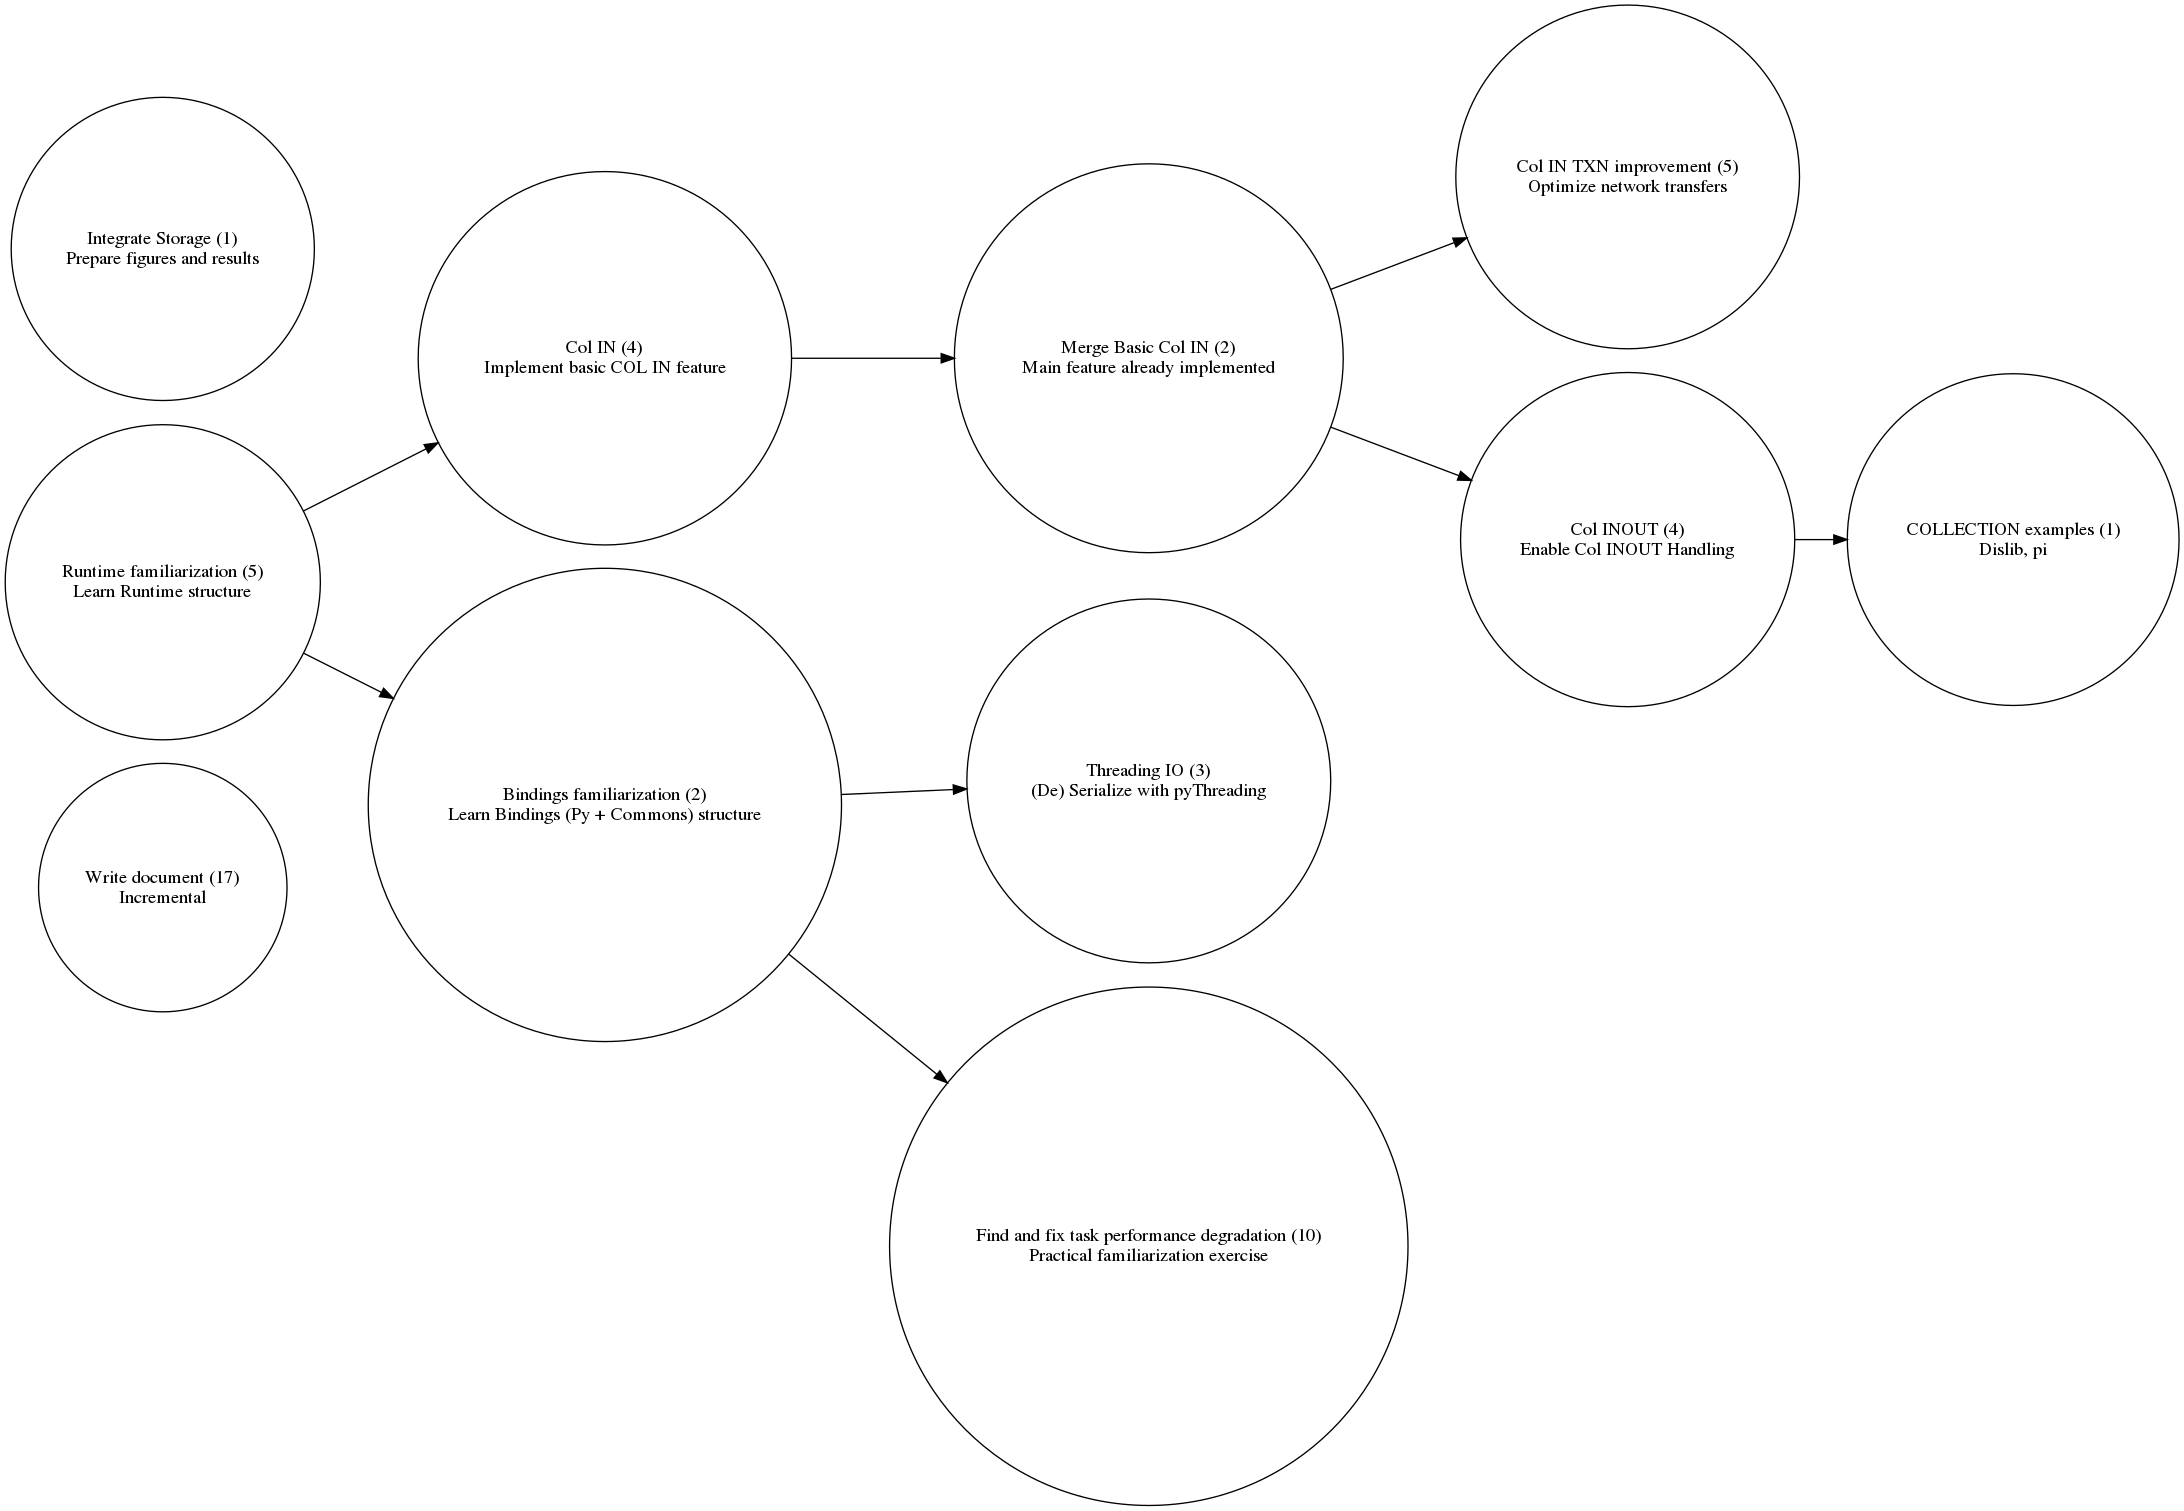
\includegraphics[scale = 0.20]{figures/thesis_task_graph.png}
\label{fig:thesis_task_graph}
\caption{A dependency graph representation of the different tasks and the dependencies between them. The numbers between parentheses denote the estimated number of needed weeks to do some task}
\end{figure}

A more precise explanation of these tasks (and shortcuts to the corresponding sections) can be found below. It is recommended to read the following sections in order to fully understand all the terms and explanations that will appear in this document.

\begin{itemize}
\item \textbf{Runtime familiarization} Some features require a deep knowledge of the COMPSs Runtime. COMPSs is written in Java, so this task will mainly consist of learning the class hierarchy and modules of the Runtime, how to build and deploy it, and how to fix and add features to it. This task is explained and developed mainly in section \ref{subsec:runtime_structure}

\item \textbf{Bindings familiarization} COMPSs has two bindings that allow the user to write applications for both C/C++ and Python. We will mainly focus on the Python (PyCOMPSs) part. This task will consist of learning the different Python modules, how user code is decorated from there, and how this binding communicates with the COMPSs Runtime via C++ Python extensions \footnote{https://docs.python.org/3/extending/building.html} and the JNI library \footnote{https://es.wikipedia.org/wiki/Java\_Native\_Interface}. The development of this task can be found in section \ref{subsec:pycompss_structure}.

\item \textbf{Collection IN} This feature will allow the user to deal with multiple COMPSs parameters at once if he puts them in some container. This task and all the others that have something to do with it is developed and explained in section \ref{sec:col}.

\item \textbf{Merge Collection IN} This task consists of integrating the changes made in COMPSs to support collections into the main branch of the software while guaranteeing that this integration does not affect the stability and performance of the software. This section includes to implement some kind of unit test, and to include it in a continuous integration environment. COMPSs has many concurrent developers attacking many sections of the software at the same time, and the software has many lines of source code, so this task may no be as trivial as it seems.

\item \textbf{Collection INOUT} Same as collection IN, but allowing inout objects as the content of a collection.

\item \textbf{Collection TXN improvement} The fact that two objects belong to the same collection can be used to our advantage to implement some improvements in how this data is transferred to the destination node. For example, they could be transferred together and then split in the destination. This idea may result in better performance (less simultaneous connections, less bandwith bottleneck) or may make things worse (less parallelism when transferring data between nodes). This last section must be considered as an extra, as the difficulty and the required time to implement it is probably out of the scope and resources of this project.

\item \textbf{Combine Storage with PyCOMPSs} One of our approaches towards the improvement of object management is to partially delegate it to some \textit{dedicated} storage backend. This includes the development of some PyCOMPSs API that allows the user to use this backend and to integrate it to the \textit{intelligence} of the COMPSs Runtime. All the work related with this task can be found in section \ref{sec:storage}.

\item \textbf{Threading IO in PyCOMPSs} Most Python implementations have a Global Interpreter Lock (GIL) that prevent parallelism with Python threads. This does not mean that some speedup can be obtained if IO operations are done with Python threads, and that Python programs are necessary sequential or, at best, concurrent (for example, the Numpy library has many linear algebra operations implemented with OpenMP). This task explores if it is worthy to parallelize IO operations with Python threads and it can be found in section \ref{sec:threading_io}.

\item \textbf{Find and fix task performance degradation} This task is just a practical exercise aimed to check if we have actually achieved a good enough understanding of the COMPSs programming model. It consists of dealing with a performance decay in a user's application. By dealing we mean to identify the problem, its sources, think about a solution and implement it (if applies). This task is developed in section \ref{sec:task_overhead}. This task is intended to serve as an extension of the explanation on how COMPSs works.

\end{itemize}

\section{Methodology}
This project will be developed in a constant-feedback, results-driven model. That is, the outcome of some implementation may make our initial planning change, as these implementations may reveal more interesting lines, or heavy limitations to the current ones.\\
\\
One of the key aspects of this kind of work is to keep results reachable and easy to reproduce. For this purpose all the contents regarding to this project can be found in two git repositories:
\begin{itemize}
\item \verb|https://github.com/srgrr/TFM| The repository with this document, and all the applications, code snippets and figures contained in it
\item \verb|https://github.com/bsc-wdc/compss| The public mirror of the COMPSs programming model. All executions and applications will contain a reference to the exact commit or tag we used
\end{itemize}
This methodology allows our reviewers to easily reproduce all the experiments and to refer to some pieces of source code mentioned here.\\
\\
All tasks are tracked and annotated in a Trello board. Trello \footnote{https://trello.com/} is an online platform that emulates the classical board with post-its on it. A screenshot depicting the Trello board can be found in figure \ref{fig:trello}.

\begin{figure}
\centering
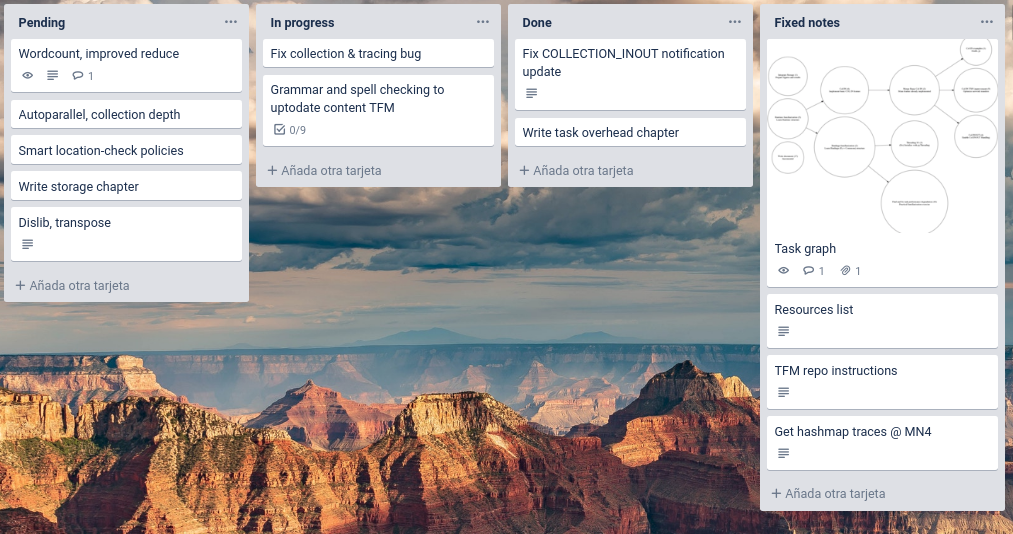
\includegraphics[scale = 0.5]{figures/trello.png}
\caption{A screenshot of the Trello board. Tasks are divided in Pending (tasks we want to do but we are not currently doing), In Progress (tasks we want to do and we are currently doing), and Done (tasks we already did but we want to comment them with our supervisors or other members of our team). We also have some fixed notes with links to useful resources, rules of the project, the task graph, and so on}
\label{fig:trello}
\end{figure}
% COLLAPSED IN A SUBSECTION
%\newpage
%\section{Document Structure}
\label{sec:doc_structure}

\section{State of The Art}
\label{sec:state_of_the_art}

\subsection{COMPSs}
\label{subsec:compss_state_of_the_art}
\section{The COMPSs Programming Model}
\label{sec:compss}
\subsection{Introduction}
COMP Superscalar (and, from now on, COMPSs) is a framework aimed to ease the development of applications for distributed infrastructures \cite{compss} \cite{Lordan2014}. A COMPSs application is typically a normal application with some special annotations and a few extra function calls in its code that transform a sequential code into a program that can run in a distributed environment.\\
\\
COMPSs applications can be written in Java, C/C++, and in Python (both 2 and 3). The Python framework is called PyCOMPSs \cite{pycompss}. All the examples and real-world usages in this project will be developed in the PyCOMPSs framework and in the Python language. However, this does not mean that all the features discussed and developed in this project are only available for PyCOMPSs. In fact, given how COMPSs is designed, the implementation of a feature for PyCOMPSs usually implies to implicitly implement it for any of the programming languages that are supported by COMPSs.\\
\\
The COMPSs framework also provides users and developers with some tools and data that helps to monitor and to debug the applications and COMPSs itself. From a user point of view, a graph of the workflow and traces of the execution of applications can be generated (figures \ref{fig:graph_example}  and \ref{fig:trace_example}). Traces are generated with a combination of Extrae \footnote{https://tools.bsc.es/doc/pdf/extrae.pdf}, Paraver \cite{paraver}, and a custom implementation inside COMPSs itself. From a developer point of view, many debug information, as logging messages and stack traces, is available if runnning COMPSs with debug flags or in case COMPSs crashes. We must mention that these logs are not always the answer or the solution. For example, if both the master and some worker complain in their respective logs about something some questions should be answered. Some questions, as knowing if some error is the cause or the consequence of some other error that happened elsewhere, are very hard to find and they may take a lot of time to be fixed.  Some of these questions, as knowing which error happened first (assuming they are independent), are even harder to answer \cite{Lamport}. 

\begin{figure}[ht!]
\centering
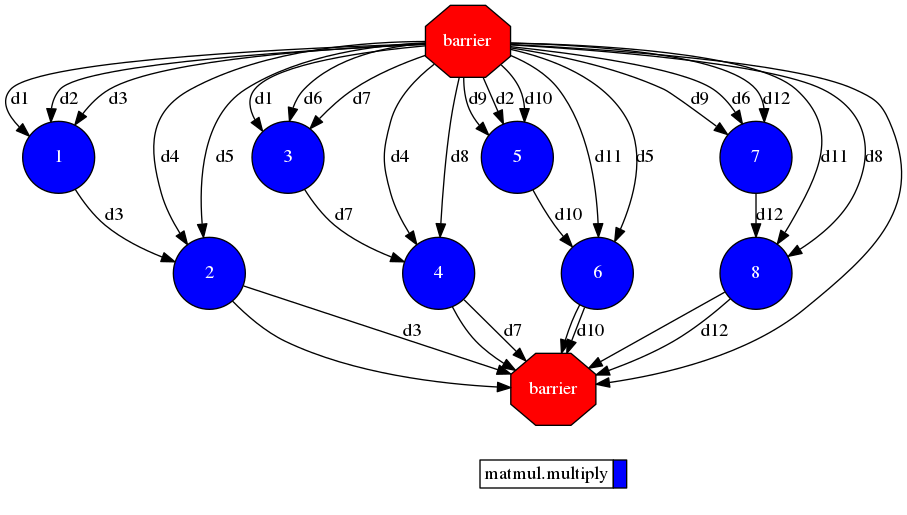
\includegraphics[scale = 0.45]{figures/2x2_matmul_graph.png}
\caption{A dependency graph generated by a COMPSs application. Circular nodes are tasks, octogonal edges are syncpoints, and edges are dependencies between tasks and/or syncpoints caused by some data. The labels of the edges are the identifiers of the data that causes these dependencies.}
\label{fig:graph_example}
\end{figure}

\begin{figure}[ht!]
\centering
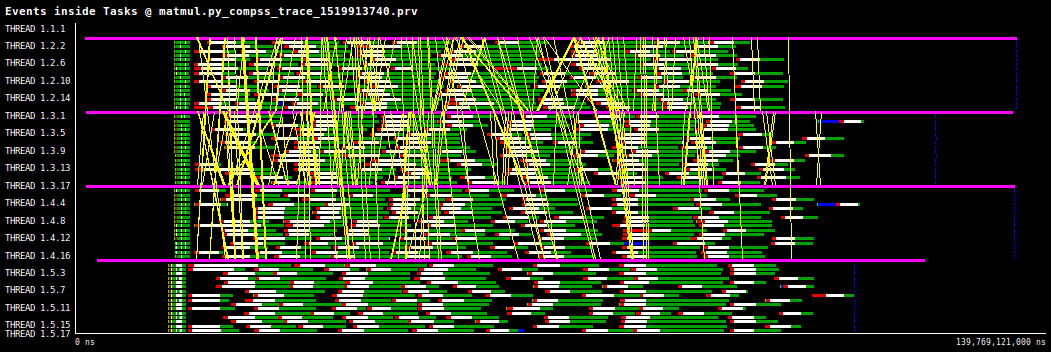
\includegraphics[scale = 0.3]{figures/matmul_trace.png}
\caption{A trace generated by a COMPSs application. Each row corresponds to a process, colored segments are different tasks, and yellow lines are network transfers between different computing nodes.}
\label{fig:trace_example}
\end{figure}

\newpage
\subsubsection{A Full Example}
\label{subsec:compss_example}
This section intends to give the reader a more or less extensive insight on what writing a COMPSs application is. We think that this section may help to \textit{materialize} concepts and will avoid to give this document an excessively abstract tone.\\
\\
Lets suppose that we want to approximate the value of $\pi$. For this purpose we have thought on a simple, randomized algorithm:
\begin{enumerate}
\item Generate $N$ random 2D points with coordinates between $-1$ and $1$
\item Consider the set of points $S$ within distance $1$ or less to the origin
\item Assume that $\frac{|S|}{N} = \frac{\pi}{4}$
\end{enumerate}

\begin{figure}[ht!]
\centering
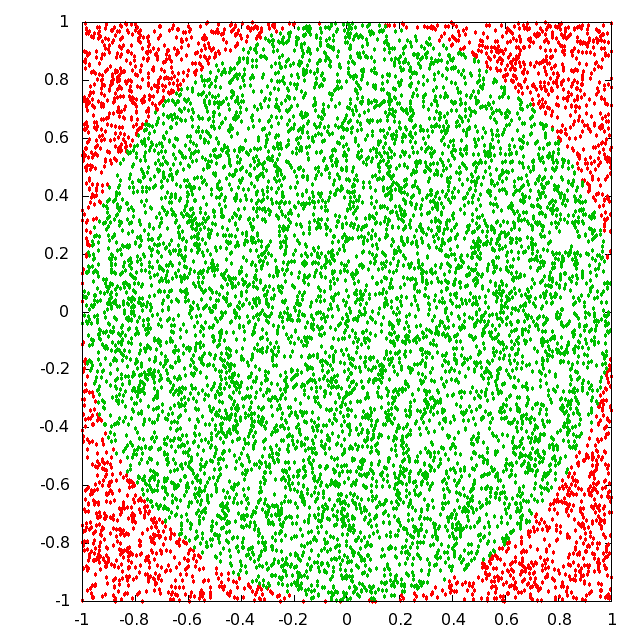
\includegraphics[scale=0.5]{figures/circle_square.png}
\caption{A graphical representation of the random experiment. The square has side length $2$, so the circle has radius $1$, and therefore area $\pi$. In ratio terms, $\frac{\pi}{4}$ of the points belong to the circle}
\label{fig:circle_square}
\end{figure}

A more graphical explanation on why this works can be found in figure \ref{fig:circle_square}.\\
\\
We know a little bit of Python, so we have decided to implement this program in it. Basically, our small application will consist of a \verb|test_random_point| function that generates a random point and return $1$ if this point lies inside our circle, and $0$ otherwise. We will call this function $N$ times, and consider the proportion $\frac{|S|}{N}$ to be equal to $\frac{\pi}{4}$.
\inputminted{python}{applications/PI_SQUARE/sequential.py}
This code can be straightforward \textit{optimized} by transforming the \verb|test_random_point| function into a COMPSs task and syncing the results in the main procedure.
\inputminted{python}{applications/PI_SQUARE/pycompss_naive.py}
Although this may be a good approach to \textit{parallelize} this application we must note that we want to make it run in a distributed environment. The main difference we can appreciate is that a COMPSs task may run in a different machine than the master code, so some coordination between two processes in different machines and the transfer of potentially big amounts of data are necessary. In other words, the tradeoff between task granularity and performance is much more punishing in distributed computing than in single-machine parallel cases.\\
\\
Another important thing to note is that a distributed application can still exploit lower level parallelism in each of its tasks. In our case, we can transform our \verb|test_random_point| function into a \verb|test_random_points| procedure that generates and tests various random points at the same time.

\inputminted{python}{applications/PI_SQUARE/pycompss_vectorized.py}

This last approach is what we consider a well \textit{COMPSsfied} application: it has a reasonable task count and granularity, and it exploits various levels of parallelism at the same time. This application also delegates most of the work to \verb|numpy| procedures, which are mainly written in C++ and OpenMP. This aspect is also important in PyCOMPSs, as Python is, by nature, a very slow programming language and it should be only used as an orchestrator.

As we mentioned in section \ref{subsec:mare_nostrum}, COMPSs is mainly designed to run in HPC environments. Most of HPC machines integrate some sort of queue system to manage its resources among all the demanding users. Our previous example can be run as a job in a queue system with the following command:

\inputminted{bash}{applications/PI_SQUARE/run_mn4.sh}

The \verb|enqueue_compss| command refers to a generic queueing script (see section \ref{subsec:hpc_queues}) which translates our request to enqueue this COMPSs job to a specific queue system. Some of the most common parameters of a COMPSs job can be found in table \ref{table:compss_queue_param}.\\
\\
\begin{table}[ht!]
\centering
\begin{tabular}{|l|l|}
\hline
Argument name   & Description                                                                           \\ \hline
\verb|exec_time|      & Job time limit                                                                        \\ \hline
\verb|num_nodes|      & \begin{tabular}[c]{@{}l@{}}Number of computing\\ nodes\end{tabular}                   \\ \hline
\verb|cpus_per_node| & \begin{tabular}[c]{@{}l@{}}Number of cores per\\ computing node\end{tabular}          \\ \hline
\verb|constraints|     & \begin{tabular}[c]{@{}l@{}}Additional constraints\\ (e.g: highmem nodes)\end{tabular} \\ \hline
\end{tabular}
\caption{Some example configuration parameters of the queue system. These parameters are usually passed as flags to the enqueue\_compss script.}
\label{table:compss_queue_param}
\end{table}


\subsection{COMPSs Components}
\label{subsec:compss_components}
COMPSs is designed, developed, and deployed in a modular way. This has some advantages:
\begin{itemize} 
\item Easier isolation of features
\item Partial COMPSs installations are possible (e.g: install COMPSs without PyCOMPSs)
\item Components can be individually replaced, leading to faster deployments
\end{itemize}
An overview of the main COMPSs components can be found in figure \ref{fig:compss_modules}. These components are also modularized, as seen in figures \ref{fig:runtime_modules} and \ref{fig:pycompss_modules}.
\begin{figure}
\centering
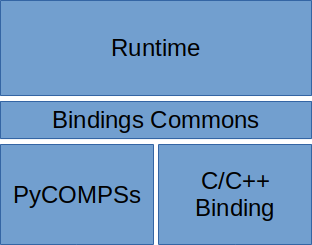
\includegraphics{figures/compss_modules.png}
\caption{Overview of the main COMPSs components.}
\label{fig:compss_modules}
\end{figure}

\begin{figure}
\centering
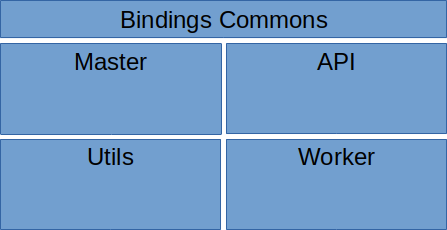
\includegraphics{figures/pycompss_modules.png}
\caption{Overview of the main PyCOMPSs components.}
\label{fig:pycompss_modules}
\end{figure}

This design choice also brings some unwanted problems. The main issue is isolation and concentration of knowledge of some parts in some developers, which leads to unnecessary code replication, lack of coherence of design and implementation choices between different modules, partial feature implementations (e.g: a feature that is only available in PyCOMPSs because it was developed by someone who did not know how to implement it in the Java runtime), and many other things. All these issues will be adressed and referred to in this document, as they appear and play an important role in our own design choices and implementations.

%TODO
\subsection{Runtime Structure}
\label{subsec:runtime_structure}

\begin{figure}
\centering
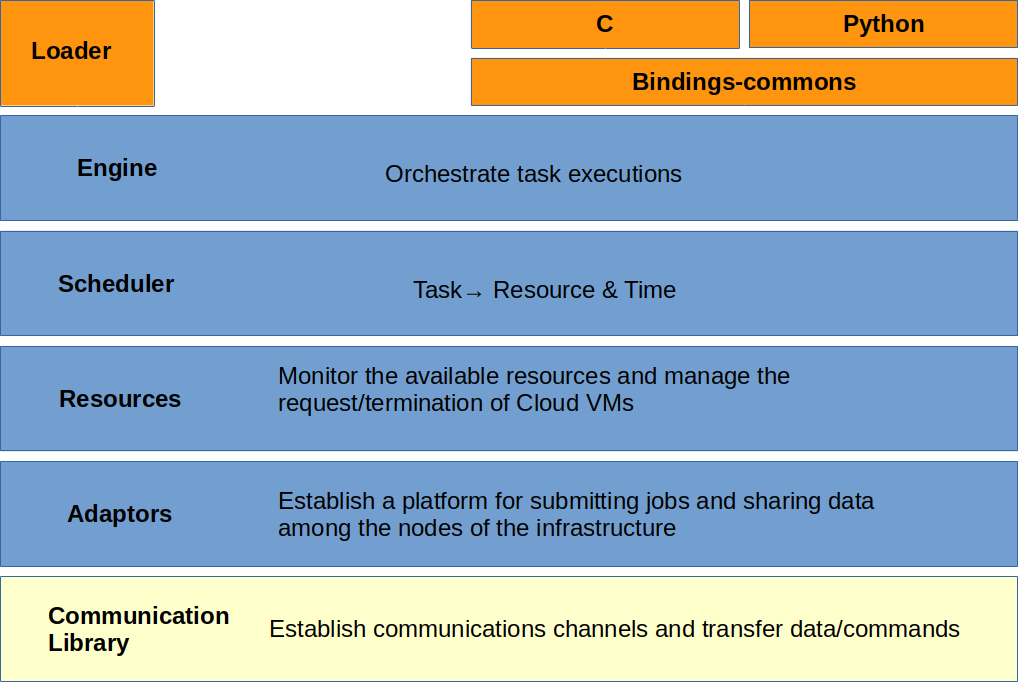
\includegraphics[scale = 0.45]{figures/runtime_modules.png}
\caption{Overview of the main Runtime components.}
\label{fig:runtime_modules}
\end{figure}

\subsection{PyCOMPSs Structure}
\label{subsec:pycompss_structure}
PyCOMPSs can be summarized as a Python Binding for COMPSs. It gives the user a way to annotate his Python code, and it internally transforms and forwards all the derived task creation requests and data to the COMPSs Runtime. Its role can be summarized as follows:
\begin{enumerate}
\item Execute the user code, both the master and the worker part
\item Implement code annotations (\verb|@task|, \verb|@binary|, etc)
\item Implement flow control mechanisms (\verb|compss_wait_on|, \verb|compss_barrier|, etc)
\item Transform the user data into something easily to transport between different machines
\end{enumerate}

\subsection{Usability vs Performance}
\label{subsec:compss_ux_vs_perf}
COMPSs has two goals: to give the not-so-expert user an easy way to make their sequential applications run in distributed environments, and to do it as efficiently as possible. Many improvements in the COMPSs framework are aimed to improve only one of these two aspects. For example, any improvement in the communication library may improve the performance of the user application, but the user will still face the same usability limitations when using COMPSs. Adding an automatic return completion, to handle the case when the user forgot to annotate the return value of some task, may save the user a lot of debugging time, but it will have no impact in the performance of the user application.\\
\\
The COMPSs software is developed and mantained by a research team in a research center, so it may be natural to think that most of the efforts and improvements are aimed to test and develop methods, models, and algorithms that improve performance, memory usage, minimize network transfers and so on. However, COMPSs is also used by other research teams as a \textit{tool} for their own purposes. Some of these teams intend to run exotic, old, complicated applications in distributed environments. Also, these teams are usually composed of researchers from different fields than computer science, so a lack of knowledge in parallel and distributed applications should be expected. The user-oriented features intend to help these research teams, and to make their life easier in the very complicated world of distributed computing. These two big forces (being a research team and having \textit{clients}) act as the main source of ideas and features in the COMPSs environments, and they are not always acting towards the same direction.\\
\\
This project tries to bring something that improves COMPSs in these two directions: give something to the user that makes his life easier while making COMPSs more efficient. For example, we do not intend to limit ourselves to give the user a way to pack some parameters in a collection. We see this feature as an opportunity to give COMPSs additional intelligence that may help to improve the performance of the framework. The same applies with the storage interface. Our goal is twofold: to give the user a way to make his or her COMPSs application run with other storage systems and to take advantage of these systems in terms of performance.


\subsection{Redis}
\label{subsec:redis_state_of_the_art}
Redis \footnote{https://redis.io/} is a 

\subsection{DataClay}
\label{subsec:dataclay_state_of_the_art}
DataClay \cite{DataClay} is a 

\subsection{Hecuba}
\label{subsec:hecuba_state_of_the_art}
Hecuba \cite{alomar2015hecuba} is a 

\subsection{Mare Nostrum IV}
\label{subsec:mare_nostrum}
%TODO: MENCIONAR QUE COMPSS ESTA PENSADO PARA SER USADO AQUI
Mare Nostrum IV is the fourth version of the Mare Nostrum supercomputer. Mare Nostrum is a generic name to refer to the main supercomputer of the Barcelona Supercomputing Center \footnote{https://www.bsc.es}.

\subsection{Queue Systems (SLURM and LSF)}
\label{subsec:hpc_queues}
Most supercomputers have many concurrent users. All of these users want to use some of the resources of the supercomputer, and usually in a selfish manner. This situation creates a lot of conflicts between users, and even some unethical behaviors such as some user killing the processes of other users. Also, many benchmarks and experiments require no noise introduced by concurrent, unrelated processes running in the same machine, so resource exclusivity must be guaranteed in these cases.\\
\\
The most common solution to the two aforementioned problems is to divide the different nodes of a supercomputer into login nodes and computing nodes. When a user opens a session in some supercomputer he will \textit{land} into some login node. Computing nodes are unreachable or even not visible by regular users, and the only way to have access to them is to ask the system for resources and wait until the system lends them to the user. The most common implementation of this resource assignment mechanism is a queue system. A queue system processes all the requests from the users, gives them a priority as a function of various parameters and lends them the requested resources according to these priorities, as a process scheduler does with processes in an operative system.\\
\\
Two of the most common queue systems are LSF \cite{zhou1992lsf} and SLURM \cite{yoo2003slurm}. All the experiments of this project will be done in the Mare Nostrum 4 supercomputer, which uses SLURM.\\
\\
Although SLURM has its own micro-language and instructions, such as \verb|srun|, and submissions scripts, most of the experiments done in this project will not need them, as we will have generic queueing scripts available to us. A generic queueing script is a script capable to work with various queue systems to generate the corresponding specific queueing scripts. In our case, our script will translate our orders into a bunch of \verb|srun| commands and similar.\\

% MOVED TO STATE OF THE ART
%\section{High Performance Computing Environments}
\label{sec:hpcenv}

\subsection{A Brief Introduction to Supercomputers}
\label{subsec:intro_sc}

\subsection{Supercomputers and Queue Systems}
\label{subsec:hpc_queues}
Most supercomputers have many concurrent users. All of these users want to use some of the resources of the supercomputer, and usually in a selfish manner. This situation creates a lot of conflicts between users, and even some unethical behaviors such as killing the processes of other users. Also, many benchmarks and experiments require no noise introduced by concurrent, unrelated processes running in the same machine, so resource exclusivity must be guaranteed in these cases.\\
\\
The most common solution to the two aforementioned problems is to divide the different nodes of a supercomputer into login nodes and computing nodes. When a user opens a session in some supercomputer he will \textit{land} into some login node. Computing nodes are unreachable or even not visible by regular users, and the only way to have access to them is to ask the system for resources and wait until the system lends them to the user. The most common implementation of this resource assignment mechanism is a queue system. A queue system processes all the requests from the users, gives them a priority as a function of various parameters and lends them the requested resources according to these priorities, as a process scheduler does with processes and processors. In our project we will use generic scripts to enqueue all of our experiments.\\
\\
Two of the most common queue systems are LSF \cite{zhou1992lsf} and SLURM \cite{yoo2003slurm}. All the experiments of this project will be done in the Mare Nostrum 4 supercomputer, which uses SLURM.\\
\\
Although SLURM has its own micro-language and instructions, such as \verb|srun|, and submissions scripts, most of the experiments done in this project will not need them, as we will have generic queueing scripts available to us. A generic queueing script is a script capable to work with various queue systems to generate the corresponding specific queueing scripts. In our case, our script will translate our orders into a bunch of \verb|srun| commands and similar.
% TODO: REFER TO ENQUEUE COMPSS IN COMPSS SECTION
% MOVED TO STATE OF THE ART
%\section{The COMPSs Programming Model}
\label{sec:compss}
\subsection{Introduction}
COMP Superscalar (and, from now on, COMPSs) is a framework aimed to ease the development of applications for distributed infrastructures \cite{compss} \cite{Lordan2014}. A COMPSs application is typically a normal application with some special annotations and a few extra function calls in its code that transform a sequential code into a program that can run in a distributed environment.\\
\\
COMPSs applications can be written in Java, C/C++, and in Python (both 2 and 3). The Python framework is called PyCOMPSs \cite{pycompss}. All the examples and real-world usages in this project will be developed in the PyCOMPSs framework and in the Python language. However, this does not mean that all the features discussed and developed in this project are only available for PyCOMPSs. In fact, given how COMPSs is designed, the implementation of a feature for PyCOMPSs usually implies to implicitly implement it for any of the programming languages that are supported by COMPSs.\\
\\
The COMPSs framework also provides users and developers with some tools and data that helps to monitor and to debug the applications and COMPSs itself. From a user point of view, a graph of the workflow and traces of the execution of applications can be generated (figures \ref{fig:graph_example}  and \ref{fig:trace_example}). Traces are generated with a combination of Extrae \footnote{https://tools.bsc.es/doc/pdf/extrae.pdf}, Paraver \cite{paraver}, and a custom implementation inside COMPSs itself. From a developer point of view, many debug information, as logging messages and stack traces, is available if runnning COMPSs with debug flags or in case COMPSs crashes. We must mention that these logs are not always the answer or the solution. For example, if both the master and some worker complain in their respective logs about something some questions should be answered. Some questions, as knowing if some error is the cause or the consequence of some other error that happened elsewhere, are very hard to find and they may take a lot of time to be fixed.  Some of these questions, as knowing which error happened first (assuming they are independent), are even harder to answer \cite{Lamport}. 

\begin{figure}[ht!]
\centering
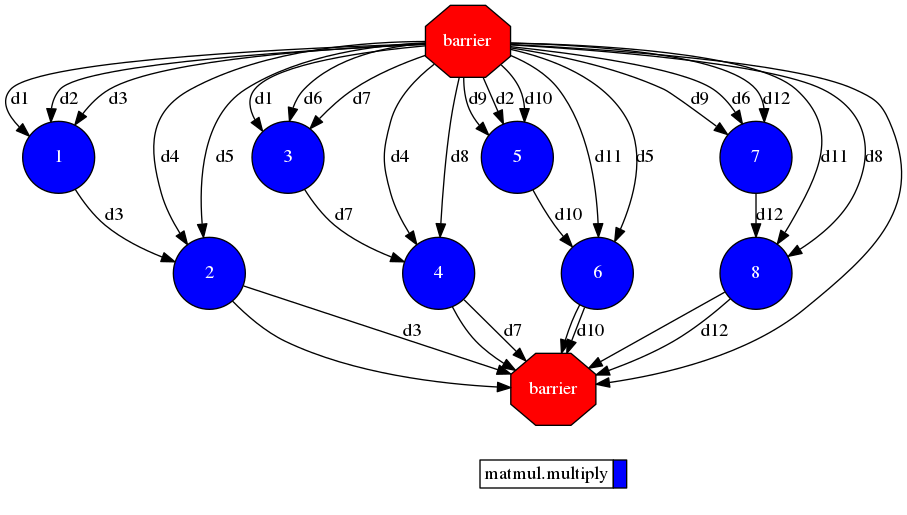
\includegraphics[scale = 0.45]{figures/2x2_matmul_graph.png}
\caption{A dependency graph generated by a COMPSs application. Circular nodes are tasks, octogonal edges are syncpoints, and edges are dependencies between tasks and/or syncpoints caused by some data. The labels of the edges are the identifiers of the data that causes these dependencies.}
\label{fig:graph_example}
\end{figure}

\begin{figure}[ht!]
\centering
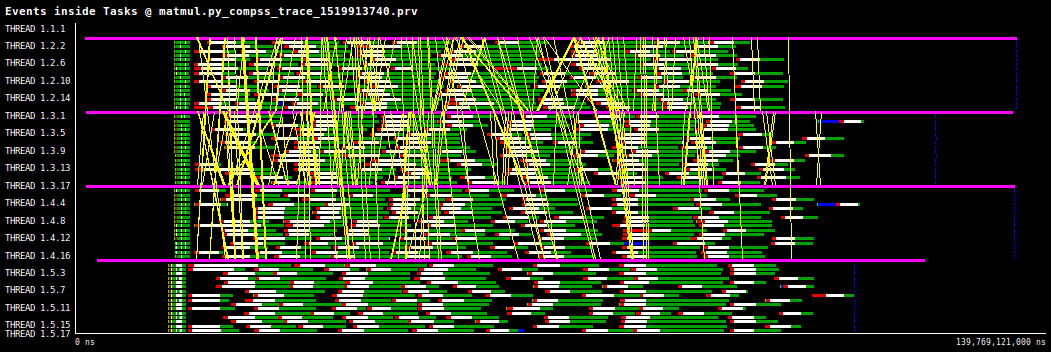
\includegraphics[scale = 0.3]{figures/matmul_trace.png}
\caption{A trace generated by a COMPSs application. Each row corresponds to a process, colored segments are different tasks, and yellow lines are network transfers between different computing nodes.}
\label{fig:trace_example}
\end{figure}

\newpage
\subsubsection{A Full Example}
\label{subsec:compss_example}
This section intends to give the reader a more or less extensive insight on what writing a COMPSs application is. We think that this section may help to \textit{materialize} concepts and will avoid to give this document an excessively abstract tone.\\
\\
Lets suppose that we want to approximate the value of $\pi$. For this purpose we have thought on a simple, randomized algorithm:
\begin{enumerate}
\item Generate $N$ random 2D points with coordinates between $-1$ and $1$
\item Consider the set of points $S$ within distance $1$ or less to the origin
\item Assume that $\frac{|S|}{N} = \frac{\pi}{4}$
\end{enumerate}

\begin{figure}[ht!]
\centering
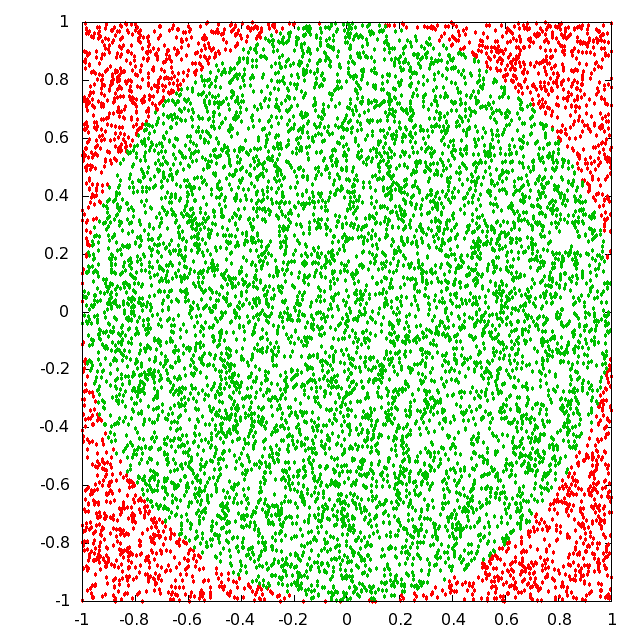
\includegraphics[scale=0.5]{figures/circle_square.png}
\caption{A graphical representation of the random experiment. The square has side length $2$, so the circle has radius $1$, and therefore area $\pi$. In ratio terms, $\frac{\pi}{4}$ of the points belong to the circle}
\label{fig:circle_square}
\end{figure}

A more graphical explanation on why this works can be found in figure \ref{fig:circle_square}.\\
\\
We know a little bit of Python, so we have decided to implement this program in it. Basically, our small application will consist of a \verb|test_random_point| function that generates a random point and return $1$ if this point lies inside our circle, and $0$ otherwise. We will call this function $N$ times, and consider the proportion $\frac{|S|}{N}$ to be equal to $\frac{\pi}{4}$.
\inputminted{python}{applications/PI_SQUARE/sequential.py}
This code can be straightforward \textit{optimized} by transforming the \verb|test_random_point| function into a COMPSs task and syncing the results in the main procedure.
\inputminted{python}{applications/PI_SQUARE/pycompss_naive.py}
Although this may be a good approach to \textit{parallelize} this application we must note that we want to make it run in a distributed environment. The main difference we can appreciate is that a COMPSs task may run in a different machine than the master code, so some coordination between two processes in different machines and the transfer of potentially big amounts of data are necessary. In other words, the tradeoff between task granularity and performance is much more punishing in distributed computing than in single-machine parallel cases.\\
\\
Another important thing to note is that a distributed application can still exploit lower level parallelism in each of its tasks. In our case, we can transform our \verb|test_random_point| function into a \verb|test_random_points| procedure that generates and tests various random points at the same time.

\inputminted{python}{applications/PI_SQUARE/pycompss_vectorized.py}

This last approach is what we consider a well \textit{COMPSsfied} application: it has a reasonable task count and granularity, and it exploits various levels of parallelism at the same time. This application also delegates most of the work to \verb|numpy| procedures, which are mainly written in C++ and OpenMP. This aspect is also important in PyCOMPSs, as Python is, by nature, a very slow programming language and it should be only used as an orchestrator.

As we mentioned in section \ref{subsec:mare_nostrum}, COMPSs is mainly designed to run in HPC environments. Most of HPC machines integrate some sort of queue system to manage its resources among all the demanding users. Our previous example can be run as a job in a queue system with the following command:

\inputminted{bash}{applications/PI_SQUARE/run_mn4.sh}

The \verb|enqueue_compss| command refers to a generic queueing script (see section \ref{subsec:hpc_queues}) which translates our request to enqueue this COMPSs job to a specific queue system. Some of the most common parameters of a COMPSs job can be found in table \ref{table:compss_queue_param}.\\
\\
\begin{table}[ht!]
\centering
\begin{tabular}{|l|l|}
\hline
Argument name   & Description                                                                           \\ \hline
\verb|exec_time|      & Job time limit                                                                        \\ \hline
\verb|num_nodes|      & \begin{tabular}[c]{@{}l@{}}Number of computing\\ nodes\end{tabular}                   \\ \hline
\verb|cpus_per_node| & \begin{tabular}[c]{@{}l@{}}Number of cores per\\ computing node\end{tabular}          \\ \hline
\verb|constraints|     & \begin{tabular}[c]{@{}l@{}}Additional constraints\\ (e.g: highmem nodes)\end{tabular} \\ \hline
\end{tabular}
\caption{Some example configuration parameters of the queue system. These parameters are usually passed as flags to the enqueue\_compss script.}
\label{table:compss_queue_param}
\end{table}


\subsection{COMPSs Components}
\label{subsec:compss_components}
COMPSs is designed, developed, and deployed in a modular way. This has some advantages:
\begin{itemize} 
\item Easier isolation of features
\item Partial COMPSs installations are possible (e.g: install COMPSs without PyCOMPSs)
\item Components can be individually replaced, leading to faster deployments
\end{itemize}
An overview of the main COMPSs components can be found in figure \ref{fig:compss_modules}. These components are also modularized, as seen in figures \ref{fig:runtime_modules} and \ref{fig:pycompss_modules}.
\begin{figure}
\centering
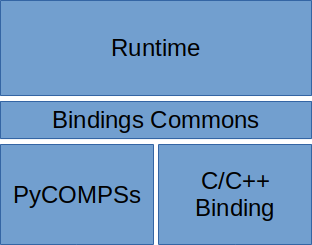
\includegraphics{figures/compss_modules.png}
\caption{Overview of the main COMPSs components.}
\label{fig:compss_modules}
\end{figure}

\begin{figure}
\centering
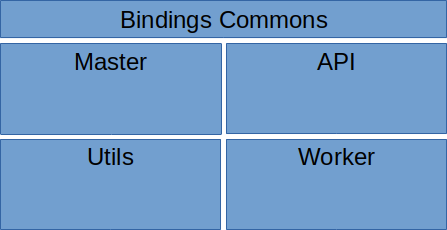
\includegraphics{figures/pycompss_modules.png}
\caption{Overview of the main PyCOMPSs components.}
\label{fig:pycompss_modules}
\end{figure}

This design choice also brings some unwanted problems. The main issue is isolation and concentration of knowledge of some parts in some developers, which leads to unnecessary code replication, lack of coherence of design and implementation choices between different modules, partial feature implementations (e.g: a feature that is only available in PyCOMPSs because it was developed by someone who did not know how to implement it in the Java runtime), and many other things. All these issues will be adressed and referred to in this document, as they appear and play an important role in our own design choices and implementations.

%TODO
\subsection{Runtime Structure}
\label{subsec:runtime_structure}

\begin{figure}
\centering
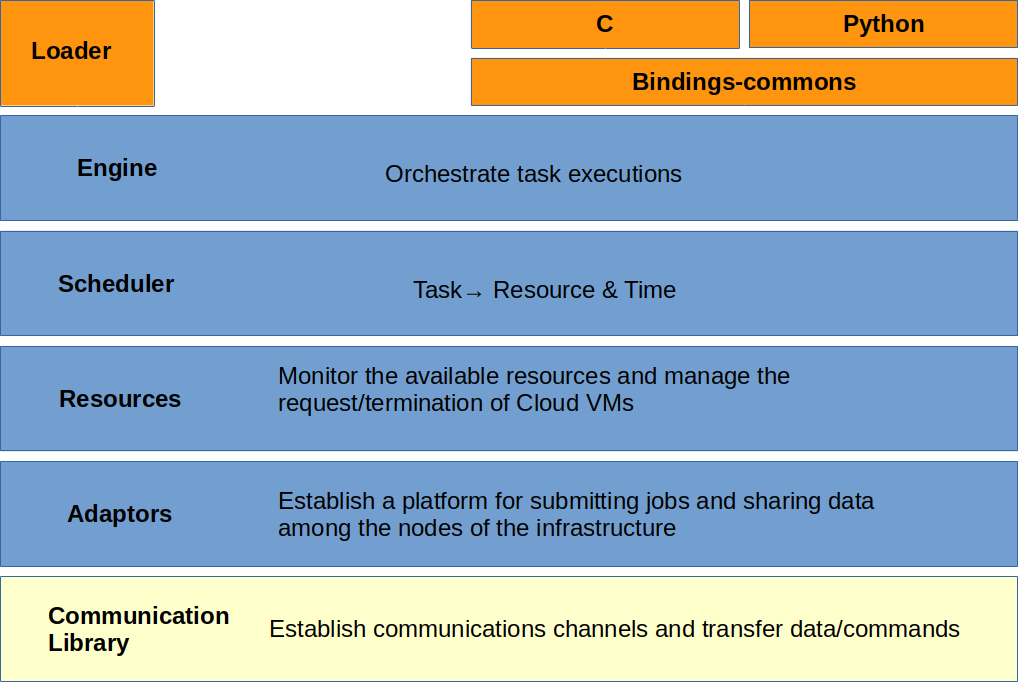
\includegraphics[scale = 0.45]{figures/runtime_modules.png}
\caption{Overview of the main Runtime components.}
\label{fig:runtime_modules}
\end{figure}

\subsection{PyCOMPSs Structure}
\label{subsec:pycompss_structure}
PyCOMPSs can be summarized as a Python Binding for COMPSs. It gives the user a way to annotate his Python code, and it internally transforms and forwards all the derived task creation requests and data to the COMPSs Runtime. Its role can be summarized as follows:
\begin{enumerate}
\item Execute the user code, both the master and the worker part
\item Implement code annotations (\verb|@task|, \verb|@binary|, etc)
\item Implement flow control mechanisms (\verb|compss_wait_on|, \verb|compss_barrier|, etc)
\item Transform the user data into something easily to transport between different machines
\end{enumerate}

\subsection{Usability vs Performance}
\label{subsec:compss_ux_vs_perf}
COMPSs has two goals: to give the not-so-expert user an easy way to make their sequential applications run in distributed environments, and to do it as efficiently as possible. Many improvements in the COMPSs framework are aimed to improve only one of these two aspects. For example, any improvement in the communication library may improve the performance of the user application, but the user will still face the same usability limitations when using COMPSs. Adding an automatic return completion, to handle the case when the user forgot to annotate the return value of some task, may save the user a lot of debugging time, but it will have no impact in the performance of the user application.\\
\\
The COMPSs software is developed and mantained by a research team in a research center, so it may be natural to think that most of the efforts and improvements are aimed to test and develop methods, models, and algorithms that improve performance, memory usage, minimize network transfers and so on. However, COMPSs is also used by other research teams as a \textit{tool} for their own purposes. Some of these teams intend to run exotic, old, complicated applications in distributed environments. Also, these teams are usually composed of researchers from different fields than computer science, so a lack of knowledge in parallel and distributed applications should be expected. The user-oriented features intend to help these research teams, and to make their life easier in the very complicated world of distributed computing. These two big forces (being a research team and having \textit{clients}) act as the main source of ideas and features in the COMPSs environments, and they are not always acting towards the same direction.\\
\\
This project tries to bring something that improves COMPSs in these two directions: give something to the user that makes his life easier while making COMPSs more efficient. For example, we do not intend to limit ourselves to give the user a way to pack some parameters in a collection. We see this feature as an opportunity to give COMPSs additional intelligence that may help to improve the performance of the framework. The same applies with the storage interface. Our goal is twofold: to give the user a way to make his or her COMPSs application run with other storage systems and to take advantage of these systems in terms of performance.

\newpage
\section{Fixing tasks overheads in PyCOMPSs}
\label{sec:task_overhead}
This first practical section describes a performance fix in the COMPSs programming model. Its intention is to give a practical example of how important is to properly manage objects in distributed programming models and to show how complex finding a bug in this kind of software can be.

\subsection{Problem description}
A COMPSs user reported via mailing list that his application showed a gradual performance degradation over time. The workflow of his application can be summarized as follows:

\inputminted{python}{applications/TASK_OVERHEAD/main.py}

The user was able to detect this performance degradation thanks to the tracing tools. Two traces showing this issue can be found in figures \ref{fig:zoom_task_early} and \ref{fig:zoom_task_late}.

\begin{figure}
\centering
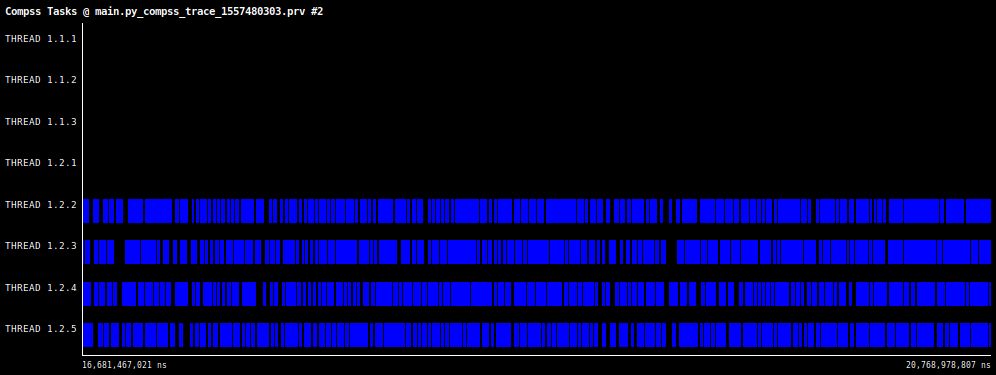
\includegraphics[scale = 0.3]{figures/zoom_task_early.png}
\caption{A trace showing the first tasks of an execution. Each row represents a thread, blue represents a task being executed and black that either the thread is waiting for the next task or it is doing something else}
\label{fig:zoom_task_early}
\end{figure}

\begin{figure}
\centering
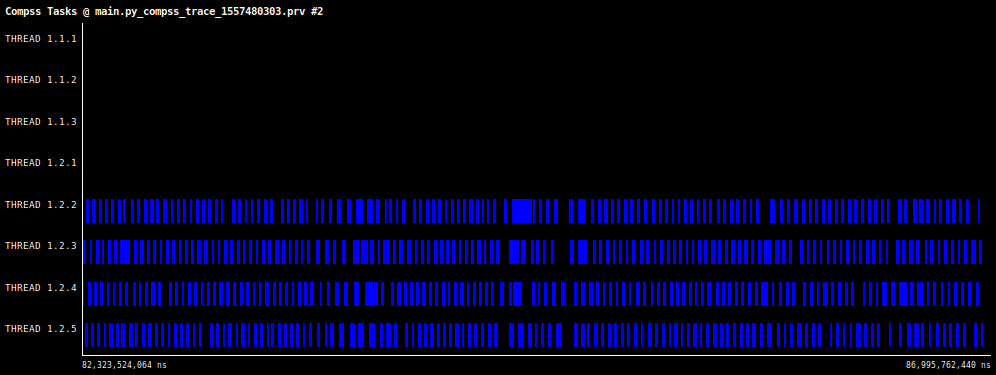
\includegraphics[scale = 0.3]{figures/zoom_task_late.png}
\caption{A trace showing the last tasks of an execution. The meaning of the trace is the same as in figure \ref{fig:zoom_task_early}, but now the spacing between tasks has increased a lot}
\label{fig:zoom_task_late}
\end{figure}

\subsection{Analysing and narrowing down the problem}
The trace from figure \ref{fig:zoom_task_late} gives us the hint that there is something wrong about how COMPSs manages tasks. Note that this fact only gives us a very rough hint on where to start looking for, but there are still many possible candidates and places to look at. Some of these places are:
\begin{itemize}
\item PyCOMPSs \verb|@task| decorator
\item PyCOMPSs object serialization
\item PyCOMPSs-to-COMPSs parameter forwarding
\item COMPSs Runtime task registering
\item COMPSs Runtime dependency computation
\item COMPSs Runtime data transfer
\item COMPSs Worker task reception
\item ...
\end{itemize}
The list may contain 30 additional items before the last(s) step(s) \textit{user's task is executed, results are serialized and the master gets a notification about it}. Some sections are arguably skippable, as our knowledge and experience tells us they cannot have anything to do with our issue, but the other ones must be revised one by one. The natural way to proceed is to simply follow the PyCOMPSs and COMPSs source code in the \textit{natural order}. That is, start from the user's source code, detect a task, go to the \verb|@task| decorator, and so on.\\
\\
Fortunately for us, the problem was on a quite early stage: the handling of the object identifiers in the Python binding.
% TODO: COMPLETE THIS SECTION, EXPLAIN HOW WE DID ARRIVE TO IDOBJ

\subsection{Object identification and mapping in PyCOMPSs}
Our first (and last) bet was on the \verb|get_object_id| function from the PyCOMPSs source code. Let's take a look at this function:

\inputminted{python}{snippets/get_object_id_old.py}

This function iterates over potentially all of the tracked objects just to get the identifier of some object (or to assign it one). This is done this way because an object needs to be hashable for being used as a key in a dictionary. Hashable usually means immutable, and no user can guarantee us that his objects will fulfill these properties. In fact, the programming model supports INOUT objects, which are, by nature, mutable objects. Some examples of mutable Python objects are \verb|[1, 2, 3, "hello"]|, \verb|object()| and \verb|numpy.random.rand(5)|.\\
\\
If the Python binding is tracking $n$ objects then this function may iterate $\mathcal{O}(n)$ times just to retrieve (or to give) a single identifier. It is not hard to see that an application with $n$ simultaneous PyCOMPSs objects will have to do $\mathcal{O}(n^2)$ iterations, which is consistent with what we observed at the traces.
\\
Even if the previous analysis tells us that there is something very wrong with this function, we still need to make sure that this is the main source of our current problem. For that purpose, we have decided to time all the calls to this function. As we can see in figure \ref{fig:task_overhead_exec_times}, this function scales pretty poorly with the number of tracked object.
\begin{figure}
\centering
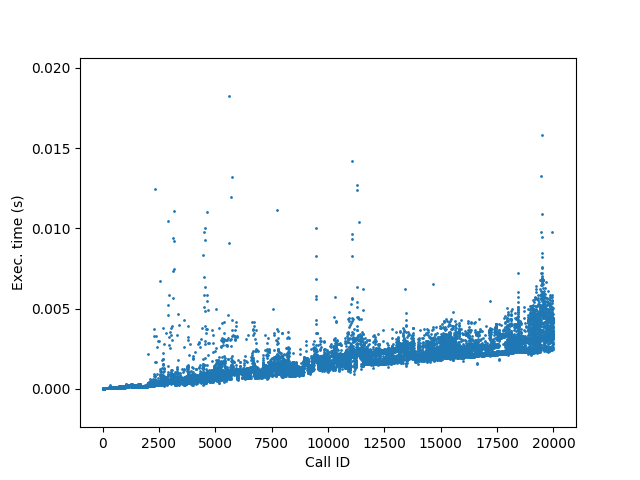
\includegraphics[scale = 0.5]{figures/task_overhead_exec_times.png}
\caption{Time required to complete a function call. Calls are arranged chronologically. Although there is a lot of noise, a linear behavior can be observed}
\label{fig:task_overhead_exec_times}
\end{figure}
All this evidence can be considered more than enough to start thinking about possible fixes and improvements. Our idea 
% TODO: ADD GRAPH OF THE PERFORMANCE DEGRADATION IN THIS FUNCTION
A possible fix may consist of using the \verb|id| function. This function accepts an object as its unique argument and returns its memory address. Note that this identifier is not entirely unique for a single object, as two objects that do not coexist may have the same memory address. However, this way to identify objects is enough for our use case. After applying this fix the \verb|get_object_id| function behaves as seen in figure \ref{fig:task_overhead_exec_times_fix}, which is the normal and expected behavior when accessing to a hashmap.

\begin{figure}
\centering
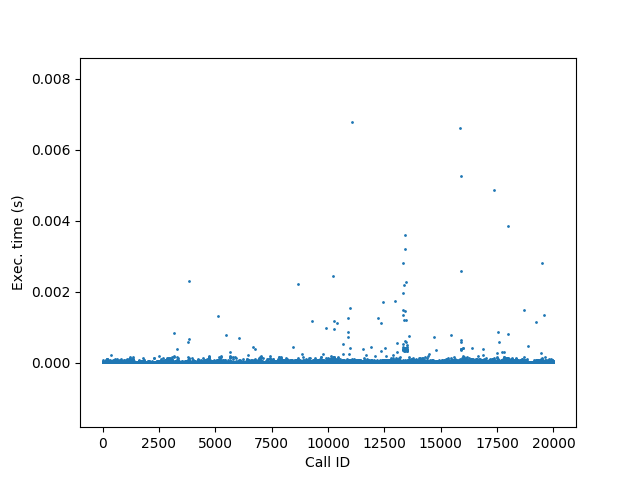
\includegraphics[scale = 0.5]{figures/task_overhead_exec_times_fix.png}
\caption{Time required to complete a function call after the fix. Call are arranged chronologically.}
\label{fig:task_overhead_exec_times_fix}
\end{figure}

Additionally, figures \ref{fig:zoom_task_early_fix} and \ref{fig:zoom_task_late_fix} show us that the time between tasks is now constant.

\begin{figure}
\centering
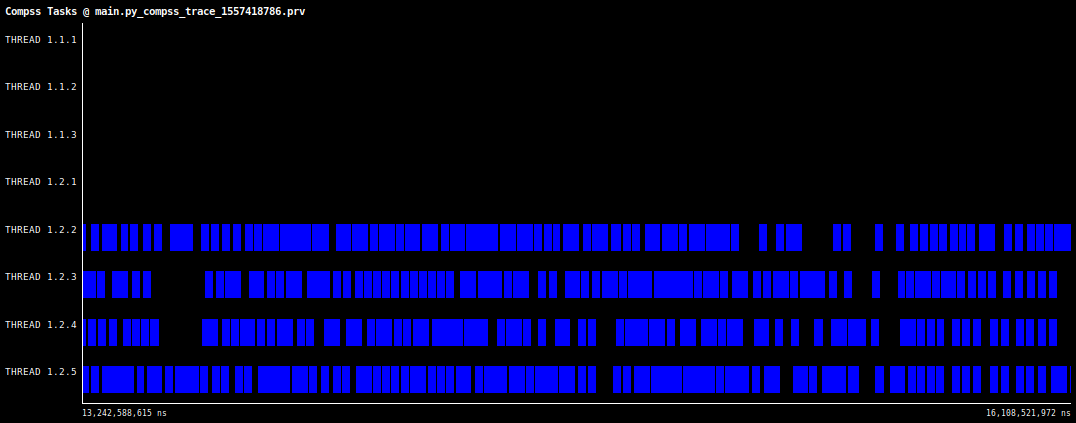
\includegraphics[scale = 0.3]{figures/zoom_task_early_fix.png}
\caption{A trace showing the first tasks of an execution after the fix. Each row represents a thread, blue represents a task being executed and black that either the thread is waiting for the next task or it is doing something else}
\label{fig:zoom_task_early_fix}
\end{figure}

\begin{figure}
\centering
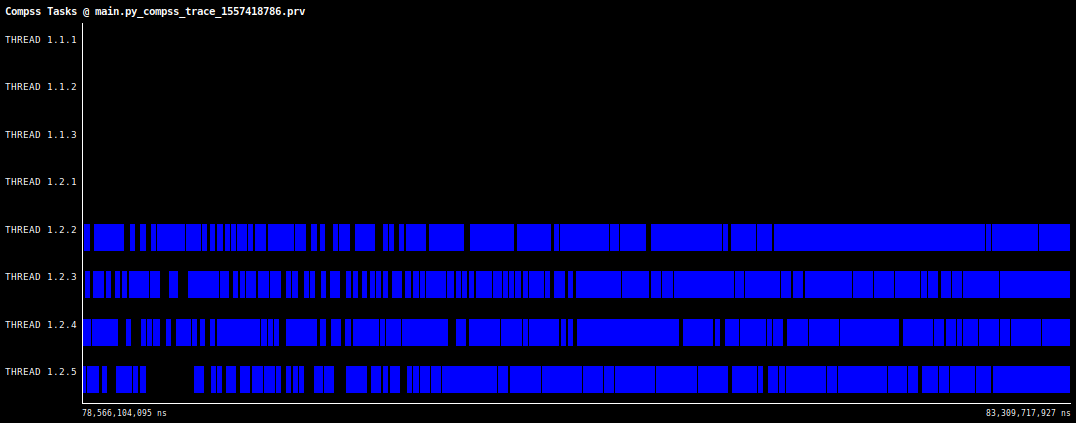
\includegraphics[scale = 0.3]{figures/zoom_task_late_fix.png}
\caption{A trace showing the last tasks of an execution after the fix. As we can see, the gaps between tasks are quite similar to the ones from figure \ref{fig:zoom_task_early_fix}}
\label{fig:zoom_task_late_fix}
\end{figure}

The overall performance gain was enourmous. Although the final implementation consisted of a few lines of source code, it was arguably hard to find where this improvement should be made. We must note that COMPSs has, according to the \verb|cloc| tool, around 300000 source lines of code (sloc).

\section{Collections in COMPSs}
\label{sec:col}
As we have seen in previous sections and examples, a COMPSs parameter is basically a regular user-code object, as a \verb|numpy.ndarray|, with additional metadata to help the COMPSs Runtime to compute any dependency between tasks induced by this particular object, keep track of its locations, and so on.\\
\\
A very common issue reported by COMPSs users is that the programming model is not able to detect dependencies induced by attributes or contents. Many examples are valid: an array \verb|[object(), some_future_object]|, an instance of a class with some attribute that is a future object... or some object that has been used in a super-object. If the container is used as a COMPSs parameter, no synchronization of the sub-object will ever happen, as the programming model won't know about it.\\
\\
The ideal solution, a generic introspection algorithm, is very hard, if not impossible, to implement. Python is dynamically typed language, some objects can be modified if iterated, many others have no easy way to list its internal attributes, circular references can happen... the list is almost endless. Another obstacle is object reconstruction. Let's consider the following code:
\begin{verbatim}
A = MyClass()
A.attribute = some_pycompss_task()
another_pycompss_task(A)
\end{verbatim}
Ideally, we would like to detect the dependency induced by \verb|A.attribute| with no synchronizations in the master, and then get the full object in the worker. This means that the programming should:
\begin{enumerate}
\item Detect the data dependency (introspection)
\item Ask for \verb|A|, and \verb|A.attribute|
\item Deserialize \verb|A| and \verb|A.attribute|, realize that one object is an attribute of the other, and add it
\end{enumerate}
These steps require a heavy implementation with a noticeable performance impact. For example, a $2000 \times 2000$ \verb|numpy.matrix| can make the programming model iterate through $4000000$ elements unnecessarily.\\
\\
However, this use case is pretty common, so something must be done. So our goal is now to determine what can be implemented within the existing time and viability constraints.\\
\\
After some meetings it was decided that support for arrays should be implemented in the COMPSs Programming Model. Given that many COMPSs users find words like \textit{array, hash map, reflection, inheritance} complicated and misleading it was decided to call this feature as \textit{support for collections}, as collection is a word that seemed more understandable by non computer science researchers. This name also gives the opportunity to extend this implementation to other iterable data structures such as sets, hash maps and so on.\\
\\
This feature should cover these two cases:
\begin{verbatim}
L = [future_object_1, future_object_2, ...]
y = f(L) # Future objects should be synced and available
\end{verbatim}

\begin{verbatim}
L = [object_1]
modify_object_1()
f(L) # object_1 should be updated and synced properly
\end{verbatim}
In other words, collections should support both IN and INOUT objects.\\
\\
This feature is especially interesting because its implementation serves two purposes: usability and performance. With no collections users are forced to use some \textit{alternative tricks} such as functions with the signature \verb|f(*args)| to deceive the programming model into believing that it is receiving multiple arguments. As we will see later, this particular trick has its own problems and issues.

\subsection{Collections as Input Parameters}
\label{subsec:col_in}
The first step consists of enabling the COMPSs Programming Model to accept collections fully composed of input parameters. This step will also help us to identify and to mark all the parts that require some implementation and/or modification when dealing with this feature.\\
\\
The easiest way to implement this feature is by what we call the \textit{contagion model}. Note that, in terms of dependencies, if some object $x$ is contained in some collection $C$ then any dependency that affects $C$ must also affect $x$, and vice versa. Let's consider the following pseudo-code:

\begin{verbatim}
c1 = f() # c1 is a future object
C = [c1, ...] # C contains a future objects and possibly more thing
g(C)
\end{verbatim}
There is a clear dependency between the function calls $g(C)$ and $f()$. The easiest way to implement this is to recursively iterate collection objects and to process each object as a single parameter. This approach still offers some room to improve performance. For example, it is not necessary to transfer certain metadata of each single element of a collection, as it can be deduced or inherited from the collection object per se. In this first case, it is not necessary to specify that the direction of all the elements $c_1, ..., c_n$ of some input collection $C$ is \verb|IN|, as it can be deduced from the fact that $C$ is an input collection.\\
\\
Once we have decided what we want to implement we must decide how and where to start. Our chosen approach is something similar to what is called TDD (Test Driven Development) \footnote{https://en.wikipedia.org/wiki/Test-driven\_development}: we wrote a PyCOMPSs app that uses collections as input parameters and now we want to make it work. The source code can be found in appendix \ref{subsec:col_in_program}.

As we mentioned in section \ref{subsec:compss_components}, the design of the programming model forces the developer to go through many layers of the software just to implement a single feature. Any PyCOMPSs parameter will go through the pipeline shown in figure \ref{fig:parameter_pipeline}.

\begin{figure}[ht!]
\centering
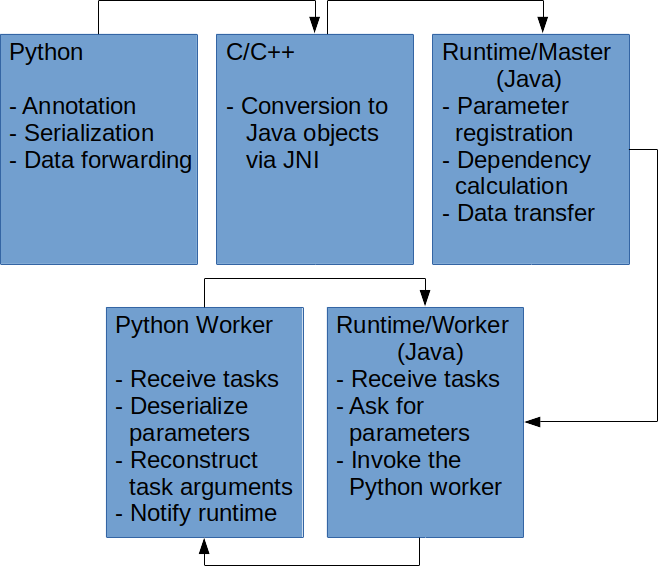
\includegraphics[scale = 0.5]{figures/parameter_pipeline.png}
\caption{The journey of a Python parameter, from the user's function call until the task is finished in the worker}
\label{fig:parameter_pipeline}
\end{figure}

Our implementation can be generalized with this pattern:

\inputminted{python}{snippets/collection_pattern.py}

This pattern allows us to implicitly define collections of collections. In fact, a \verb|Depth| field can be defined when decorating a task. This field has a default value of 1, and it determines the allowed levels of recursion before considering any object a regular COMPSs parameter. For example, if \verb|Depth = 2| and a $2 \times 2 \times 2$ matrix is passed as a parameter, COMPSs will interpret it as $2 \times 2$ collection.

\subsection{Collections as INOUT Parameters}
\label{subsec:col_inout}


\subsection{Practical Applications}
\label{subsec:col_examples}
\subsection{Approximating cardinalities of huge sets}
\label{subsec:wcountproblem}
The Count-Distinct or Word Count Problem can be formulated as follows: given a sequence of elements $s_{1}, ..., s_{n}$ compute the amount of \textbf{distinct} elements in it. For example, for the sequence dog, cat, dog, bird, bird the answer is 3 (the distinct elements are bird, cat, and dog).

If the sequence is not too large this problem can be easily solved in expected linear time and space using hash tables, or $\mathcal{O}(nlogn)$ time and linear space using some data structures as Red-Black trees. However, this bound on space starts to become unacceptable when datasets are too large. In this section we will describe a probabilistic algorithm named as HyperLogLog \cite{Flajolet07hyperloglog:the}.\\
\\
This algorithm is very simple and yet very powerful. The core idea is the following: for each element $s_{i}$ of our sequence, use a hash function $h: \{0, 1\}^{*} \mapsto \{0, 1\}^b$ to compute a value $h(s_{i})$ and estimate the cardinality as $2^m$, where $m$ is the maximum number of leading zeros among all $h(s_{i})$. We must note that if all $h(x)$ have the same probability $\frac{1}{2^{b}}$ then the probability for some value to have $k$ leading zeros is $2^{-k}$. This means that the expected number of observations that are needed to find a number with $k$ leading zeros is $2^{k}$. Given that having a single hash value is not precise enough but computing multiple hash functions is too expensive, what is done is the following: 
\begin{enumerate}
\item Given a token $t$, compute $h(t)$
\item Take the first $p$ bits and use them to refer to a position in an array consisting of $2^p$ elements $a_{0}, ..., a_{2^p - 1}$
\item Update this position according to the other $b - p$ bits so it keeps the maximum amount of leading zeros seen so far
\item Once all tokens are processed output the harmonic mean of $2^{a_{0}}, ..., 2^{a_{2^p - 1}}$ as the answer.
\end{enumerate}
An interesting trivia fact is that if we need $\mathcal{O}(\log n)$ bits for our hash function to be able to count until $n$ then we only need $\mathcal{O}(\log \log n)$ to store the number of leading zeros of some hash value. This is why HyperLogLog is called that way.\\
\\
A very nice property of HyperLogLog is that two distinct runs on two different datasets can be merged if they have used the same parameters (hash function, $b$, and $p$) in such a way that it approximates the cardinality of the union of the two datasets. Given two arrays $a$ and $b$, each corresponding to a run of HyperLogLog we can get a fictional run of HyperLogLog $c$ that represents the union of both datasets by computing $c_{i} =\max(a_{i}, b_{i})$ for all of the $2^{p}$ positions. This makes sense, as it produces the same result as running a single HyperLogLog on the concatenation of the two datasets. This property allows us to parallelize or to distribute this algorithm, giving us a potential performance boost. The source code we will use for our experiments can be found in appendix \ref{subsec:hyperloglog_source_code}.\\
\\
Note that this application is a classical \textit{map-reduce} workflow. Without collections we are forced to implement any reduce function as \verb|reduce(f, *args)|. Each extra argument is passed as an input parameter via socket and pipe, implying a huge overhead. With collections only the collection object, and the list of identifiers, are transferred. The other properties of the contents, such as direction, locations and so on, are deduced or requested in the destination node.\\
\\
The elimination of this overhead is noticeable even with a very small number of parameters. As we can see in figure \ref{fig:collection_vs_normal}, the collection feature reduces the overhead drastically. An important observation is that a PyCOMPSs task of the form \verb|f(*args)| usually starts to show problems and crashes when more than $60$ arguments are passed, as each argument represents a lot of metadata to be transferred via socket and pipe.
\begin{figure}[ht!]
\centering
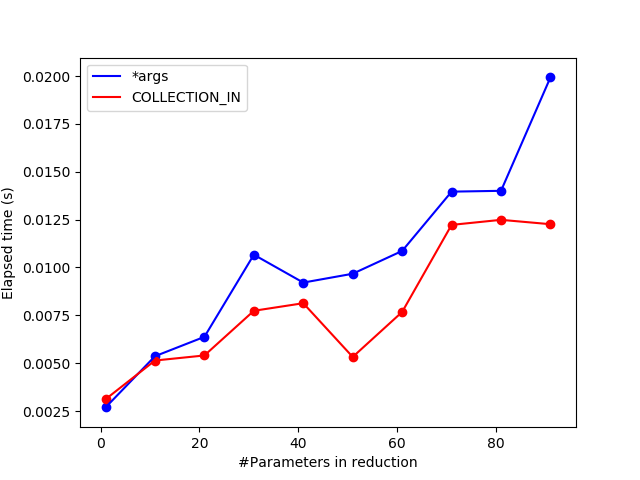
\includegraphics[scale = 0.5]{figures/collection_vs_normal.png}
\caption{Execution time of the reduce functions with and without collections. Each point is the average of 5 executions. Although the samples are noisy, as they are small, a consistent improvement by the collection feature can be appreciated. The non-collections versions started to crash and to show strange behaviours around the 60 parameters}
\label{fig:collection_vs_normal}
\end{figure}\\
\\
A comparison between the amount of meta-data generated and sent by the classical reduce implementation and by the collections version can be found in appendix \ref{subsec:reduce_data_comparison}.

This improvement benefits many applications, as the map-reduce scheme is very common.
\subsubsection{Usage of collections in other projects}
\label{subsubsec:col_projects}
%TODO: ramon exaqute
The collection feature was very welcome by some other research groups and projects. Among these research groups 
\section{Combining Storage Systems with COMPSs}
\label{sec:storage}
Most COMPSs objects are created by the user and managed by the Runtime. The data transferring software is a self-made library based on NIO \footnote{https://docs.oracle.com/javase/7/docs/api/java/nio/package-summary.html}. Although this is usually a good enough solution for most use cases, there are three scenarios in which it may be a disadvantage to use this library:

\begin{enumerate}
\item The objects are the output of some previous application
\item The outputs of the COMPSs application are the input of some other application
\item The filesystem and/or the network presents huge bandwidth limitations
\end{enumerate}

The two first items represent a common usability problem. Many research groups generate their inputs 
%TODO: FINISH THIS CHAPTER

\subsection{Defining a Storage API}
\label{subsec:storage_api}
The need of defining a storage API comes from the fact that some researchs groups are interested into mixing some of their tools with the COMPSs Programming Model. After some meetings with these groups it was decided 
%TODO: ALSO FINISH THIS ONE

\subsection{A Practical Implementation: Redis}
\label{subsec:storage_redis}
The first step towards validating this storage API consisted of providing a valid, functional implementation. For this purpose Redis was chosen.\\
\\
Redis \footnote{https://redis.io/} is a simple Key-Value distributed storage database. Redis can be seen as a distributed hash map with $2^14 = 16384$ slots. Each key is either chosen by the user or randomly assigned, and it determines the position of this object in the hash table. More precisely, given a key $k$, and a value $v$, $v$ will be stored at the position $\textrm{CRC16}(k) \mod \quad 16384$. CRC16\footnote{https://en.wikipedia.org/wiki/Cyclic\_redundancy\_check} is a known checksum-like method used by many devices and network protocols to check that a message has been sent with no errors, and it can also be used as a quick hash function.\\
\\
Our implementation serializes objects in-memory and stores them as byte arrays in the database. Although this does not save us from serializing objects it is enough to avoid dealing with the filesystem, and to do all the operations in-memory. Huge byte arrays are split in distributed blocks to avoid long-term load imbalances and to increase long-term data locality. If we have $N$ worker nodes, our data is $M$ bytes long, it is available at only one node, and nodes are busy enough to make data locality irrelevant then the expected data transferring time is
$$E_1[N] = \frac{N - 1}{N} \times M$$
If our data is split into $K$ blocks, $\frac{M}{K}$ bytes each block, and each block is at a different node then the expected data transferring time can expressed as

$$E_2[N] \leq \frac{K}{N}(K - 1)\frac{M}{K} + \frac{N - K}{N}M$$

By simplifying $M = 1$ we obtain that $E_2[N] \leq E_1[N] = \frac{N - 1}{N}$. However, this second approach offers the opportunity to introduce parallelism and, in fact, most practical applications show that the required time to transfer the $(K - 1)$ remaining blocks is usually less or equal than $2.5\frac{M}{K}$, or something around that, and that in the worst case scenario the introduced overhead is relatively negligible, which is consistent with the two formulas above.

Another detail about our Redis implementation is that Redis offers no direct way to make some piece of data end in some node. However, the Storage API defines a method which allows the user to do that. Our solution to this problem consisted of simply generating random keys until one of them mapped to a valid slot. This adds almost no overhead, as the number of nodes tends to be a very manageable number such as 16, 32, 64, or at most 128 in most practical cases.

\subsection{Practical Applications}
\label{subsec:storage_apps}
\subsubsection{K-Means}
\label{subsubsec:kmeans_redis}
K-Means \cite{Lloyd82leastsquares} is a clustering algorithm which, given $N$ $k$-dimensional points and an integer $c$, assigns each point a label between $1$ and $c$. The idea is that these labels represent groups of \textit{similar} points. An example of what this algorithm computes can be found in figure \ref{fig:kmeans_example}.

\begin{figure}
\centering
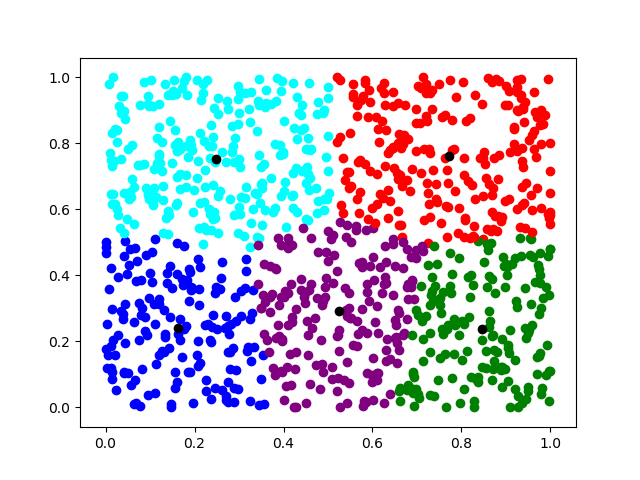
\includegraphics[scale = 0.5]{figures/kmeans_example.png}
\caption{A set of points grouped by the K-Means algorithm. Black points represent centroids, colours represent different groups}
\label{fig:kmeans_example}
\end{figure}

The algorithm can be sumarized as follows:

\begin{enumerate}
\item Generate $c$ random $d$ dimensional points, call them \textit{centroids}
\item For each point of the input data, compute the nearest centroid, assign them labels according to which centroid is the closest
\item For each group, compute the mean of its members. Use this mean point as the new centroid
\item Repeat step 2 until the new centroids are \textit{equal enough} to the old ones
\end{enumerate}

This algorithm can be easily run in distributed by dividing the input points into chunks and replicating the centroids in each computing node. Note that the input points will not vary during all the execution, and that the centroids usually represent a very small amount of data, so no big network transfers should be expected here, and therefore no huge improvements should be observed with the storage implementation. Our PyCOMPSs implementation is the following:

\inputminted{python}{snippets/kmeans_storage.py}

As we can deduce from the main loop in the \verb|kmeans_frag| function, this algorithm has no parallelism between iterations, but each iterations offers a lot of parallelism per se. A graph showing this workflow can be found in figure \ref{fig:kmeans_storage_dep_graph}.


Some results of how this application scales and behaves with various, different storage implementations and with files can be found in figures \ref{fig:kmeans_storage_dep_graph} \ref{fig:kmeans_strong_redis} \ref{fig:kmeans_strong_speedup_redis}, \ref{fig:kmeans_weak_redis}, and \ref{fig:kmeans_weak_speedup_redis}.

\begin{figure}[ht!]
\centering
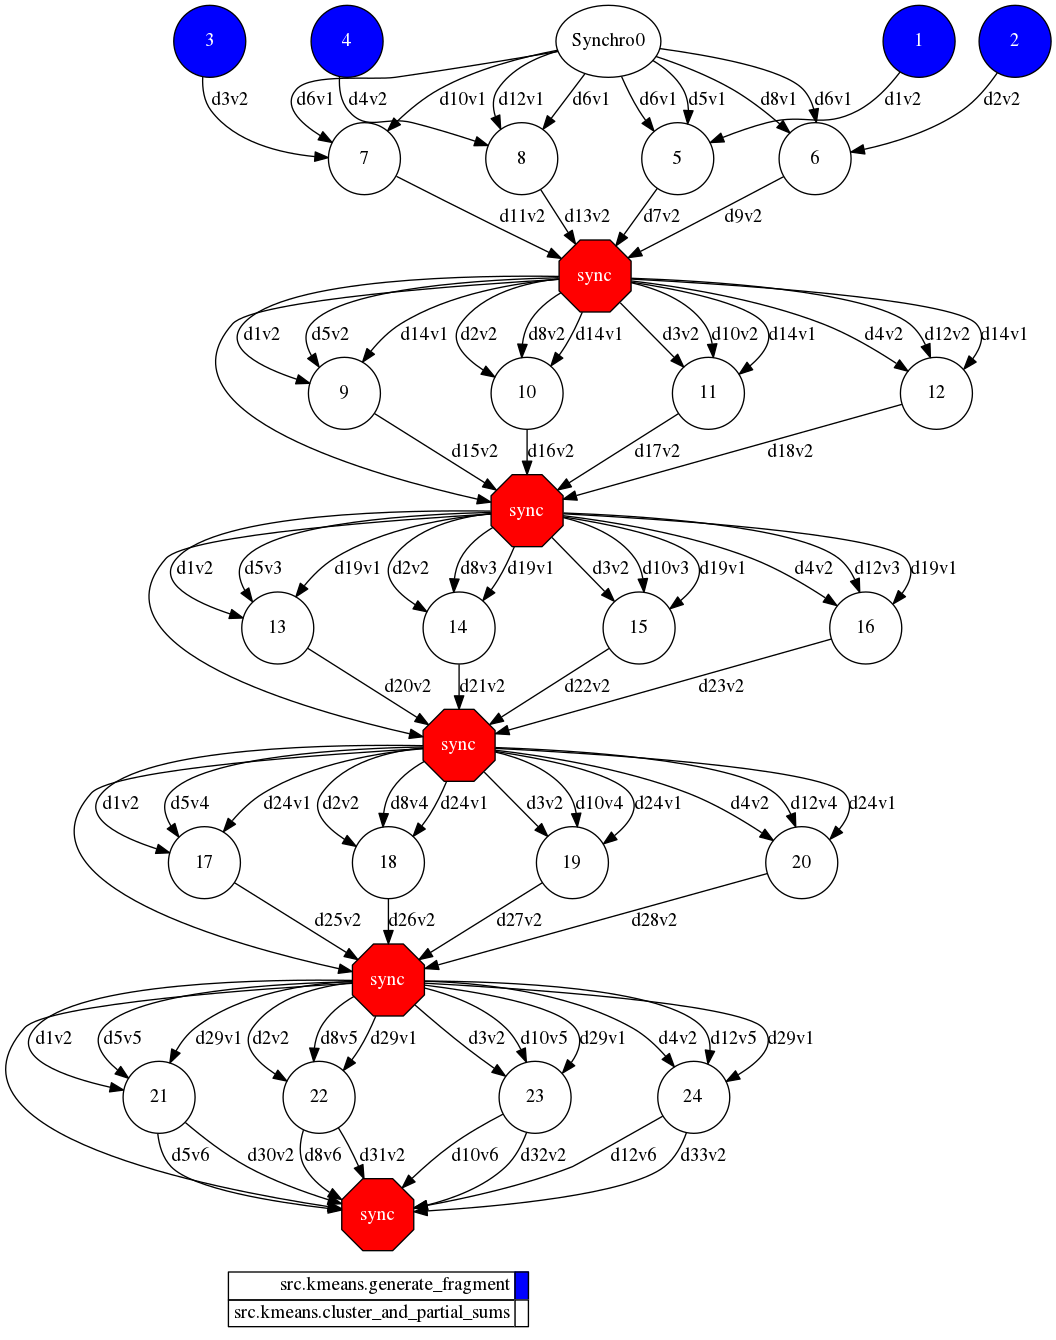
\includegraphics[scale = 0.3]{figures/kmeans_storage_dep_graph.png}
\caption{Dependency graph of a 6-iteration K-Means execution with $4$ point fragments.}
\label{fig:kmeans_storage_dep_graph}
\end{figure}

\begin{figure}[ht!]
\centering
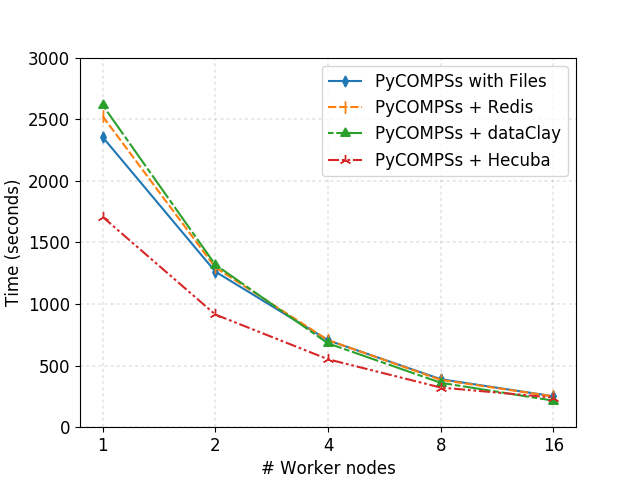
\includegraphics[scale = 0.5]{figures/storage/kmeans_strong.png}
\caption{Strong scaling graph of our various storage implementations}
\label{fig:kmeans_strong_redis}
\end{figure}


\begin{figure}[ht!]
\centering
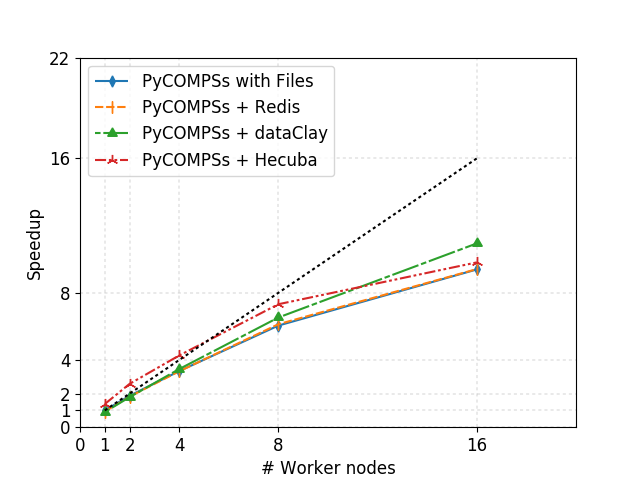
\includegraphics[scale = 0.5]{figures/storage/kmeans_strong_speedup.png}
\caption{Strong scaling speedup graph of our various storage implementations}
\label{fig:kmeans_strong_speedup_redis}
\end{figure}


\begin{figure}[ht!]
\centering
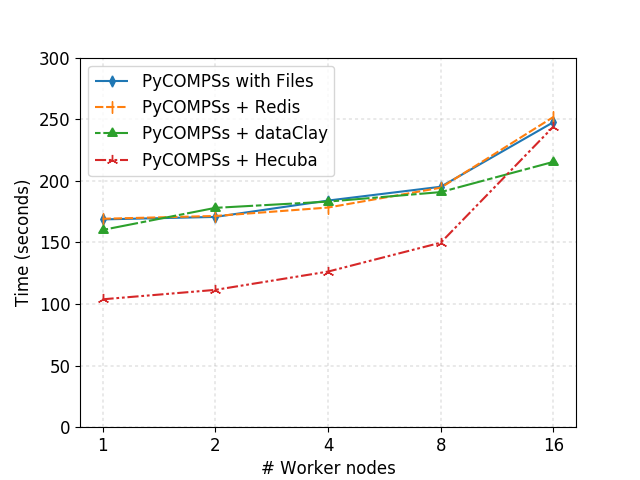
\includegraphics[scale = 0.5]{figures/storage/kmeans_weak.png}
\caption{Weak scaling graph of our various storage implementations}
\label{fig:kmeans_weak_redis}
\end{figure}


\begin{figure}[ht!]
\centering
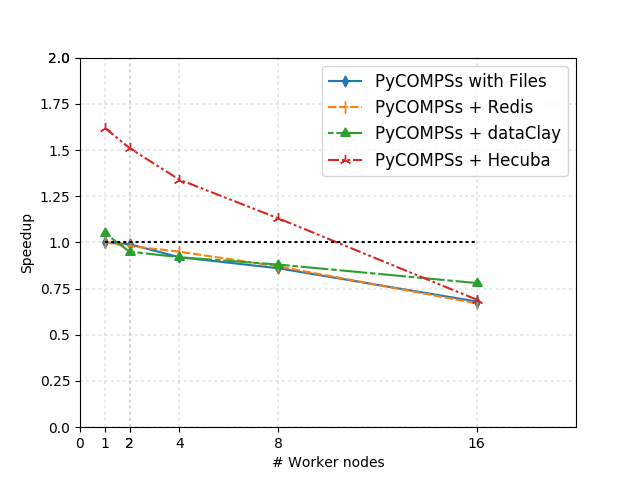
\includegraphics[scale = 0.5]{figures/storage/kmeans_weak_speedup.png}
\caption{Weak scaling speedup graph of our various storage implementations}
\label{fig:kmeans_weak_speedup_redis}
\end{figure}

As we can see, our storage implementation does not improve the overall performance of this application. However, as we can see in figure \ref{fig:kmeans_transfer_trace}, this applications has little to no heavy transfers, only at the beggining, so these results are more or less expected.


%TODO: GET THE KMEANS TRACE

\subsubsection{Matrix Multiplication}
\label{subsubsec:matmul_redis}
The matrix multiplication is a very common algorithm and it is usually the preferred example of what an embarrassingly parallel application is (i.e: a parallel application with no dependencies). Its distributed version is also interesting but due to other property: the enormous amount of required data transfers. Let's take a look to the following code:

\inputminted{python}{snippets/matmul_python.py}

This code can be parallelized in any of the three loops. The only special requirement is to make sure 



As we can see in figures \ref{fig:matmul_strong_redis} and \ref{fig:matmul_strong_speedup_redis} the Matrix Multiplication gets a huge benefit from our storage systems.

\begin{figure}
\centering
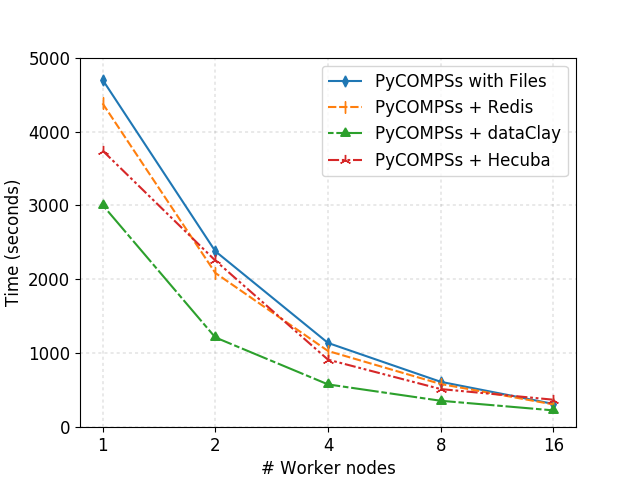
\includegraphics[scale = 0.5]{figures/storage/matmul.png}
\caption{Strong scaling graph of our various storage implementations}
\label{fig:matmul_strong_redis}
\end{figure}



\begin{figure}
\centering
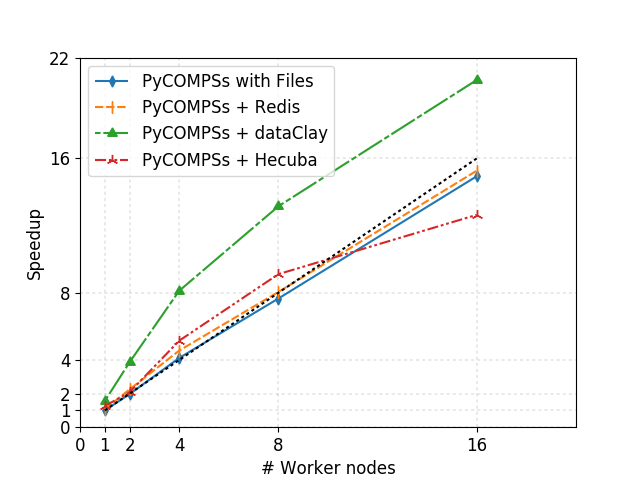
\includegraphics[scale = 0.5]{figures/storage/matmul_speedup.png}
\caption{Strong scaling speedup graph of our various storage implementations}
\label{fig:matmul_strong_speedup_redis}
\end{figure}


% LEFT AS FUTURE WORK
%\section{Parallelizing IO operations}
\label{sec:threading_io}

\section{Conclusions and Future Work}
\subsection{Conclusions}
\label{subsec:conclusions}


\subsection{Future Work}
\label{subsec:future_work}

Let's consider the application from section \ref{subsubsec:matmul_redis}. In the product of two $2 \times 2$ matrices the dependency $mul(A_{1, 1}, B_{1, 1}, C_{1, 1}) \implies mul(A_{1,2}, B_{2, 1}, C_{1, 1})$ appears, when it is actually enough to ensure that no two tasks involving the same $C_{i, j}$ are executed concurrently. An open research line consists of developing a distributed mechanism that ensures task commutativity. It was discussed to implement the option to assign each task a commutativity group, meaning that two tasks that belong to this group are mutually commutative. Task commutativity is already implemented in the OMPSs programming model \cite{duran2011ompss}, but it still remains as a challenge to implement an equivalent feature for a distributed programming model. 



\appendix % Cue to tell LaTeX that the following "chapters" are Appendices
\chapter{Collections as Input Parameters}
\label{subsec:col_in_program}
\inputminted[breaklines = true]{python}{applications/COLLECTION_IN/resources_in_master.py}

\chapter{Collections as INOUT Parameters}
\label{subsec:col_inout_program}
\inputminted[breaklines = true]{python}{applications/COLLECTION_INOUT/resources_in_worker.py}

The same application but adding a task which changes a single element of a collection, proving that our recursion pattern is enough to catch the two possible ways in which dependencies are generated (from collection to content, and from content to collection).

\inputminted[breaklines = true]{python}{applications/COLLECTION_INOUT/resources_in_worker_complex_workflow.py}


\chapter{HyperLogLog}
\label{subsec:hyperloglog_source_code}
Main application:
\inputminted[breaklines = true]{python}{applications/HYPERLOGLOG/main.py}
\verb|HyperLogLog| class
\inputminted[breaklines = true]{python}{applications/HYPERLOGLOG/HyperLogLog.py}


\chapter{Metadata generation comparison}
\label{subsec:reduce_data_comparison}

A task \verb|f(a, b, c, d, e)| sends this information through a socket:
\begin{verbatim}
[BINDING-COMMONS]  -  @GS_RegisterCE  -  Task registered: metadata.f
[BINDING-COMMONS]  -  @GS_ExecuteTaskNew - Processing task execution in bindings-common. 
[BINDING-COMMONS]  -  @GS_ExecuteTaskNew  -  Processing parameter 0
[BINDING_COMMONS]  -  @process_param
[BINDING-COMMONS]  -  @process_param  -  ENUM DATA_TYPE: 9
[BINDING-COMMONS]  -  @process_param  -  File: ...
[BINDING-COMMONS]  -  @process_param  -  ENUM DIRECTION: 0
[BINDING-COMMONS]  -  @process_param  -  ENUM STREAM: 3
[BINDING-COMMONS]  -  @process_param  -  PREFIX: null
[BINDING-COMMONS]  -  @process_param  -  NAME: *args*_0
[BINDING-COMMONS]  -  @GS_ExecuteTaskNew  -  Processing parameter 1
[BINDING_COMMONS]  -  @process_param
[BINDING-COMMONS]  -  @process_param  -  ENUM DATA_TYPE: 9
[BINDING-COMMONS]  -  @process_param  -  File: ...
[BINDING-COMMONS]  -  @process_param  -  ENUM DIRECTION: 0
[BINDING-COMMONS]  -  @process_param  -  ENUM STREAM: 3
[BINDING-COMMONS]  -  @process_param  -  PREFIX: null
[BINDING-COMMONS]  -  @process_param  -  NAME: *args*_1
[BINDING-COMMONS]  -  @GS_ExecuteTaskNew  -  Processing parameter 2
[BINDING_COMMONS]  -  @process_param
[BINDING-COMMONS]  -  @process_param  -  ENUM DATA_TYPE: 9
[BINDING-COMMONS]  -  @process_param  -  File: ...
[BINDING-COMMONS]  -  @process_param  -  ENUM DIRECTION: 0
[BINDING-COMMONS]  -  @process_param  -  ENUM STREAM: 3
[BINDING-COMMONS]  -  @process_param  -  PREFIX: null
[BINDING-COMMONS]  -  @process_param  -  NAME: *args*_2
[BINDING-COMMONS]  -  @GS_ExecuteTaskNew  -  Processing parameter 3
[BINDING_COMMONS]  -  @process_param
[BINDING-COMMONS]  -  @process_param  -  ENUM DATA_TYPE: 9
[BINDING-COMMONS]  -  @process_param  -  File: ...
[BINDING-COMMONS]  -  @process_param  -  ENUM DIRECTION: 0
[BINDING-COMMONS]  -  @process_param  -  ENUM STREAM: 3
[BINDING-COMMONS]  -  @process_param  -  PREFIX: null
[BINDING-COMMONS]  -  @process_param  -  NAME: *args*_3
[BINDING-COMMONS]  -  @GS_ExecuteTaskNew  -  Processing parameter 4
[BINDING_COMMONS]  -  @process_param
[BINDING-COMMONS]  -  @process_param  -  ENUM DATA_TYPE: 9
[BINDING-COMMONS]  -  @process_param  -  File: ...
[BINDING-COMMONS]  -  @process_param  -  ENUM DIRECTION: 0
[BINDING-COMMONS]  -  @process_param  -  ENUM STREAM: 3
[BINDING-COMMONS]  -  @process_param  -  PREFIX: null
[BINDING-COMMONS]  -  @process_param  -  NAME: *args*_4
[BINDING-COMMONS]  -  @GS_ExecuteTaskNew  -  Processing parameter 5
[BINDING_COMMONS]  -  @process_param
[BINDING-COMMONS]  -  @process_param  -  ENUM DATA_TYPE: 9
[BINDING-COMMONS]  -  @process_param  -  File: ...
[BINDING-COMMONS]  -  @process_param  -  ENUM DIRECTION: 1
[BINDING-COMMONS]  -  @process_param  -  ENUM STREAM: 3
[BINDING-COMMONS]  -  @process_param  -  PREFIX: #
[BINDING-COMMONS]  -  @process_param  -  NAME: $return_0
\end{verbatim}

While the collection equivalent generates this data:

\begin{verbatim}
[BINDING-COMMONS]  -  @GS_RegisterCE  -  Task registered: metadata.g
[BINDING-COMMONS]  -  @GS_ExecuteTaskNew - Processing task execution in bindings-common. 
[BINDING-COMMONS]  -  @GS_ExecuteTaskNew  -  Processing parameter 0
[BINDING_COMMONS]  -  @process_param
[BINDING-COMMONS]  -  @process_param  -  ENUM DATA_TYPE: 26
[BINDING-COMMONS]  -  @process_param  -  Collection: ...
[BINDING-COMMONS]  -  @process_param  -  ENUM DIRECTION: 0
[BINDING-COMMONS]  -  @process_param  -  ENUM STREAM: 3
[BINDING-COMMONS]  -  @process_param  -  PREFIX: null
[BINDING-COMMONS]  -  @process_param  -  NAME: c
[BINDING-COMMONS]  -  @GS_ExecuteTaskNew  -  Processing parameter 1
[BINDING_COMMONS]  -  @process_param
[BINDING-COMMONS]  -  @process_param  -  ENUM DATA_TYPE: 9
[BINDING-COMMONS]  -  @process_param  -  File: ...
[BINDING-COMMONS]  -  @process_param  -  ENUM DIRECTION: 1
[BINDING-COMMONS]  -  @process_param  -  ENUM STREAM: 3
[BINDING-COMMONS]  -  @process_param  -  PREFIX: #
[BINDING-COMMONS]  -  @process_param  -  NAME: $return_0
\end{verbatim}

\chapter{Redis Storage API implementation}
\label{subsec:storage_api_redis_impl}
Python:
\inputminted[breaklines = true]{python}{applications/STORAGE/redisPSCO/COMPSs-Redis-bundle/python/storage/api.py}
Java:
\inputminted[breaklines = true]{java}{applications/STORAGE/redisPSCO/src/main/java/storage/StorageItf.java}
The \verb|storage_init.sh| script, used to build Redis clusters on demand:
\inputminted[breaklines = true]{bash}{applications/STORAGE/redisPSCO/scripts/storage_init.sh}

\chapter{K-Means + Storage Implementation}
\label{subsec:kmeans_redis}
\inputminted[breaklines = true]{python}{snippets/kmeans_storage.py}


\chapter{Matmul + Storage Implementation}
\label{subsec:matmul_redis}
\inputminted[breaklines = true]{python}{snippets/matmul_storage.py}
% TODO list portfolios (of yearly) for Graham and best methods (long), and between machines (short)
%\include{Appendices/AppendixC}

%----------------------------------------------------------------------------------------
%	BIBLIOGRAPHY
%----------------------------------------------------------------------------------------

\printbibliography[heading=bibintoc]

%----------------------------------------------------------------------------------------

\end{document}  
